\subsection{External Interface Requirements}
\subsubsection{User Interfaces}
\begin{enumerate}
\item[•]{\Large Data4Help}
\bigbreak
\noindent
The third parties interested in having location and health status information of individuals can make the request on the Data4Help’s Website. Since the individuals do not need any particular Data4Help’s App for their data retrievement, Data4Help does not offer any other user interface besides its Website. 
On the Website thought, for the third parties it is possible to make both group and individual requests and to view all the data provided to the specific third party. The third parties in order to send a data request must register through the registration function offered by the Website.
\bigbreak
\noindent
The following mockups represent a basic idea of what the Data4Help’s Website will look like in the first release.
\\ [2cm]
\begin{figure}[H]
\centering
\includegraphics[scale=0.3]{Images/Mockups/Grouprequest.jpg}
\caption{Group monitoring request.}
\end{figure}
\begin{figure}
\centering
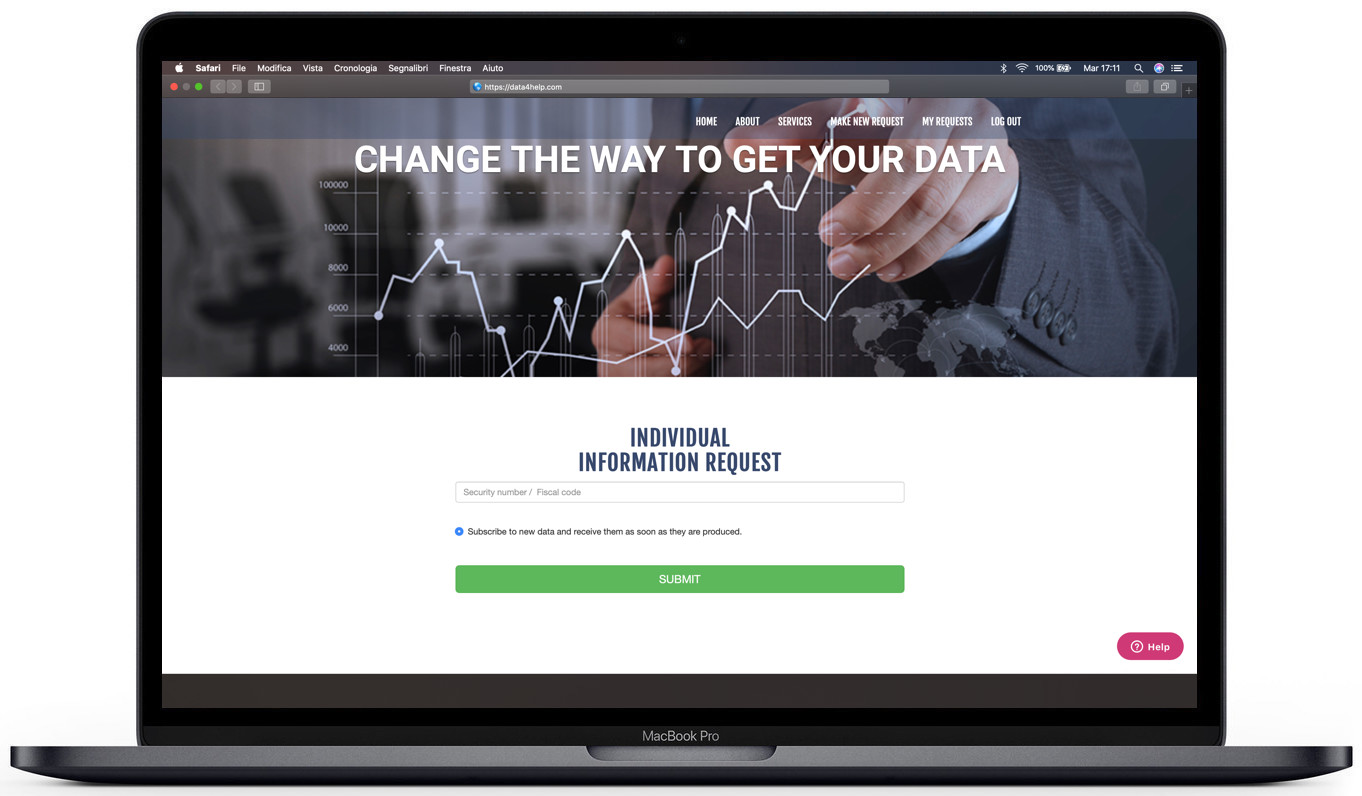
\includegraphics[scale=0.3]{Images/Mockups/IndividualRequest.jpg}
\caption{Individual monitoring request.}
\end{figure}
\newpage
\item[•]{\Large AutomatedSOS}
\bigbreak
\noindent
TrackMe offers to AutomatedSOS users an App for smartwatches, with which the users can see their location and health status information. No interface is offered to the third parties since they interact exclusively with Data4Help's Interface. 
\begin{figure}[H]
\begin{center}
        \begin{minipage}[c]{.40\textwidth}
        \centering
          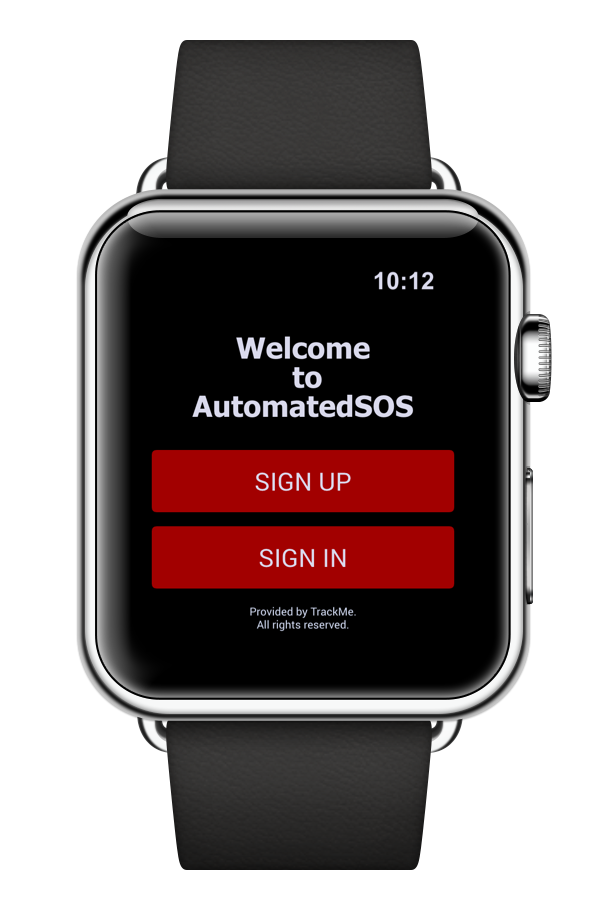
\includegraphics[height=9.3cm]{Images/Mockups/AutomatedSOSMockup1.png}
	\caption{Welcome page that the user see in the first App access. Sign up and Sign in are two possibilities.}
        \end{minipage}%
        \hspace{10mm}%
        \begin{minipage}[c]{.40\textwidth}
        \centering
          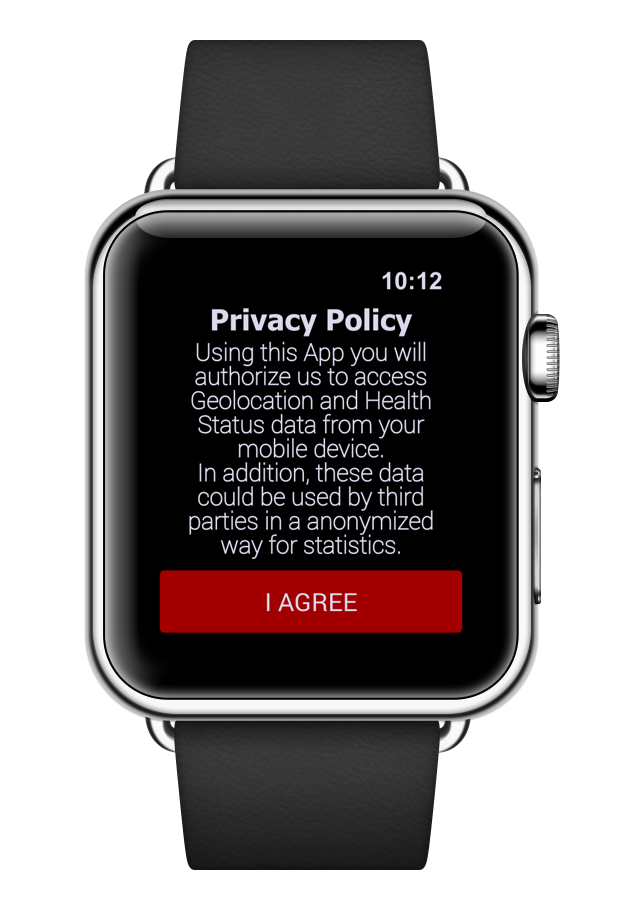
\includegraphics[height=9.3 cm]{Images/Mockups/AutomatedSOSMockup2.png}
	\caption{Privacy policy conditions regarding Data4Help's treatment of data and group monitoring request.}
        \end{minipage}
      \end{center}
\end{figure}
\begin{figure}[H]
\begin{center}
        \begin{minipage}[c]{.40\textwidth}
	\centering
          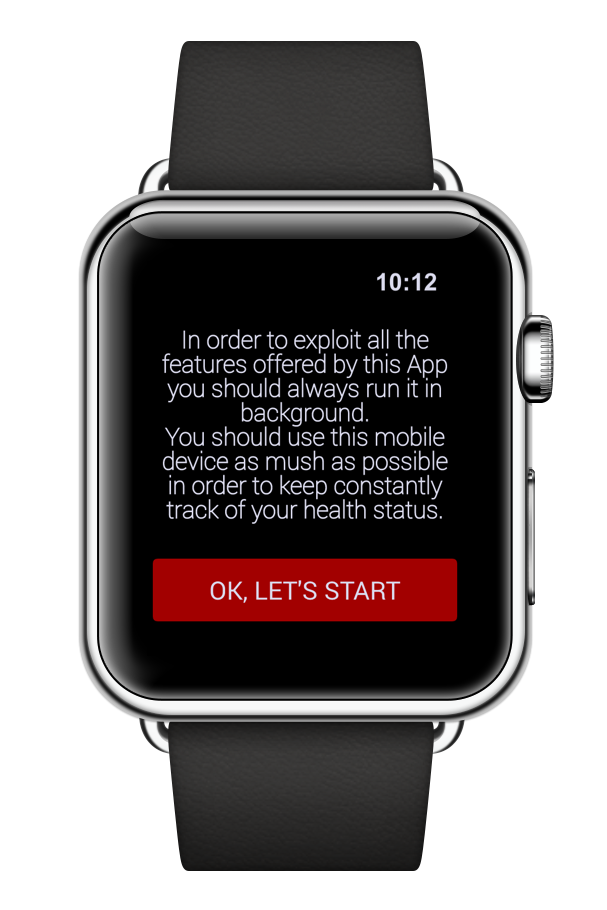
\includegraphics[height=9.5  cm]{Images/Mockups/AutomatedSOSMockup4.png}
	\caption{Message that communicates to the user the importance of wearing the smartwatch.}
        \end{minipage}%
        \hspace{10mm}%
        \begin{minipage}[c]{.40\textwidth}
	\centering
          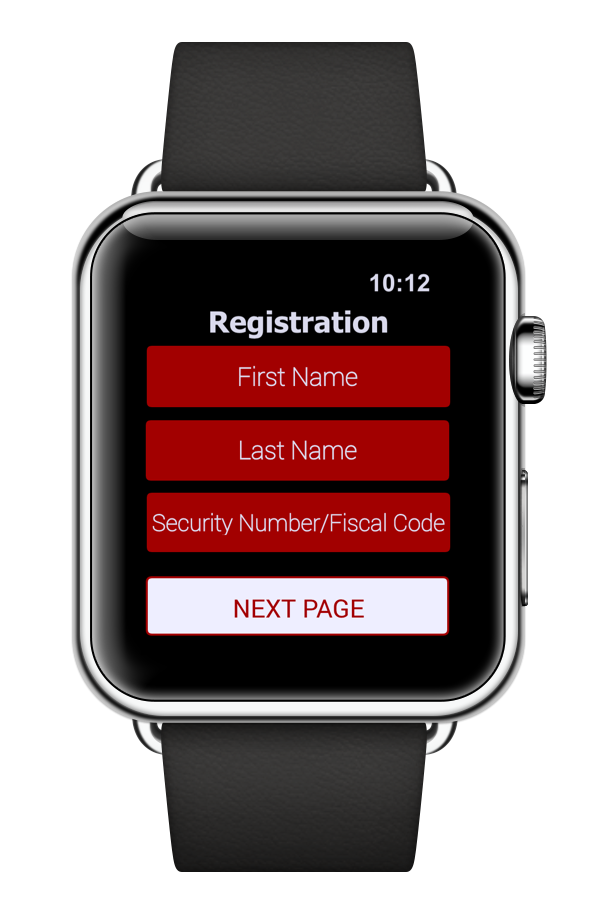
\includegraphics[height=9.5 cm]{Images/Mockups/AutomatedSOSMockup5.png}
	\caption{Main menu showing the various functions offered to user.}
        \end{minipage}
      \end{center}
\end{figure}
\begin{figure}[H]
\begin{center}
        \begin{minipage}[c]{.35\textwidth}
	\centering
          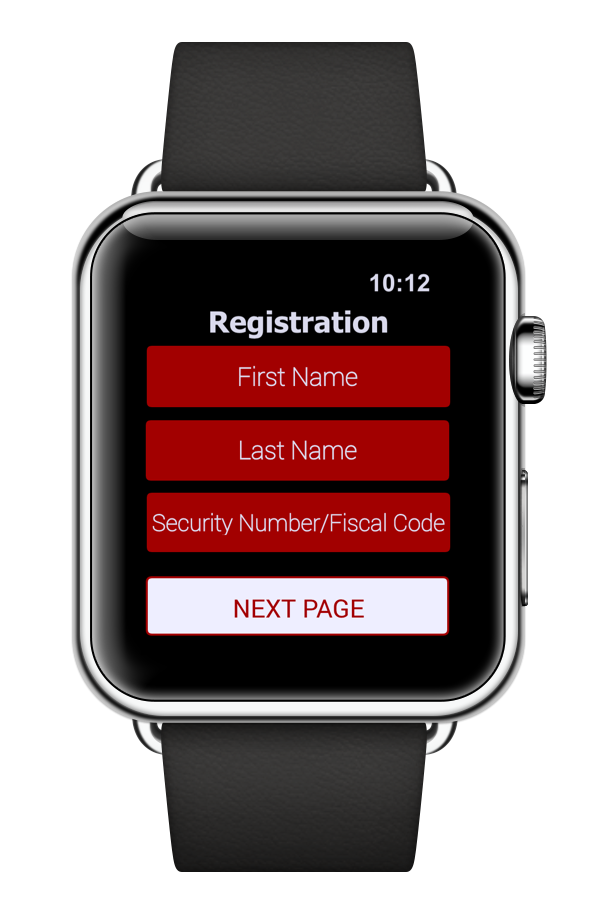
\includegraphics[height=9.5  cm]{Images/Mockups/AutomatedSOSMockup6.png}
	\caption{Fields the user have to fill to complete the registration.}
        \end{minipage}%
        \hspace{10mm}%
        \begin{minipage}[c]{.40\textwidth}
	\centering
          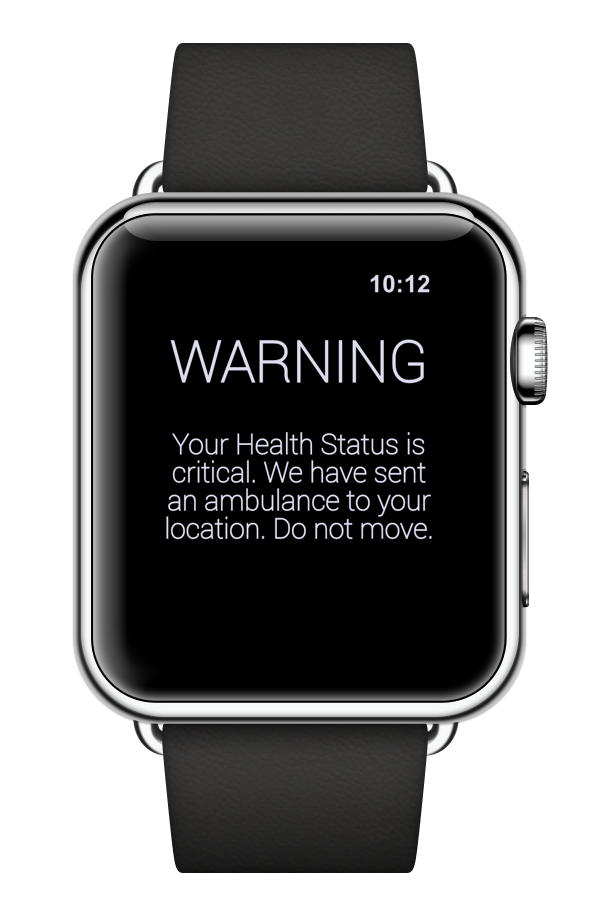
\includegraphics[height=9.5cm]{Images/Mockups/AutomatedSOSMockup7.png}
	\caption{Warning message that communicates to the user that an ambulance has been sent to the user location.}
        \end{minipage}
      \end{center}
\end{figure}

\item[•]{\Large Track4Run}
\bigbreak
\noindent
Track4Run users can use an App for smartphone and another one for smartwatches. The first one could be used by everyone, while the second one is made only for the athletes. Like for AutomatedS0S, there is not any interface provided for the third parties.
\bigbreak
\noindent
The mockups showed below represent a basic idea of what the Track4Run's App for smartphone will look like in the first release.
\\ [2cm]
\begin{figure}[H]
\begin{center}
        \begin{minipage}[c]{.40\textwidth}
        \centering
          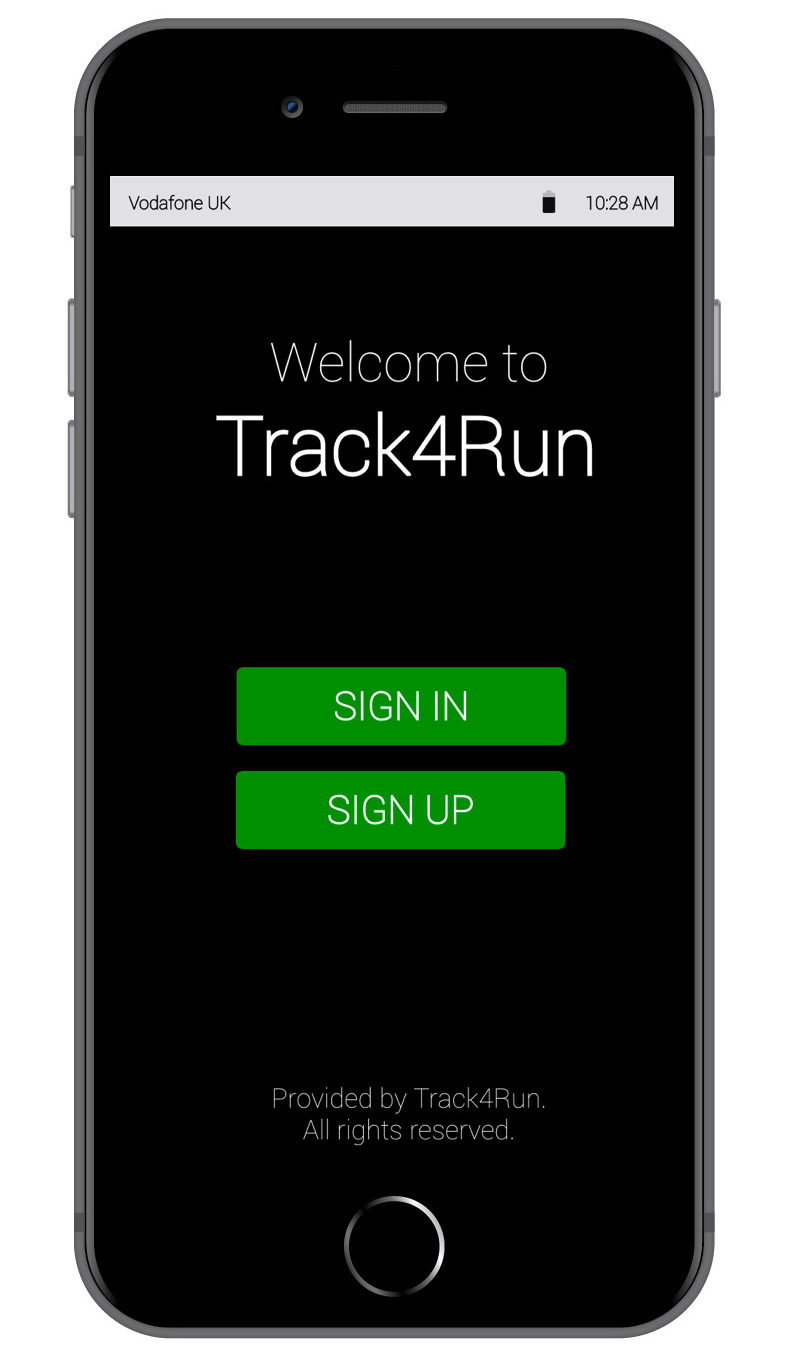
\includegraphics[height=10.4 cm]{Images/Mockups/Track4RunMockup1.jpg}
	\caption{Welcome page. }
        \end{minipage}%
        \hspace{10mm}%
        \begin{minipage}[c]{.40\textwidth}
        \centering
          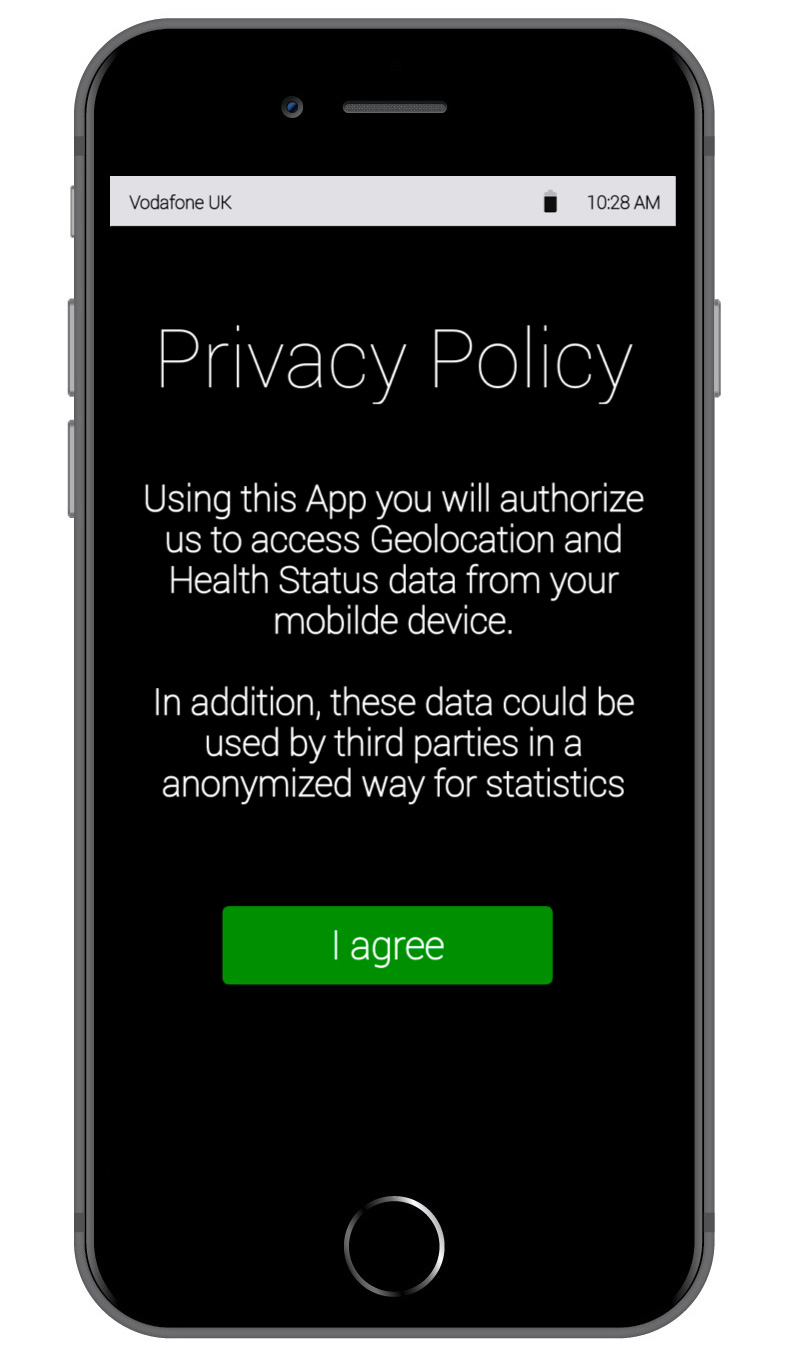
\includegraphics[height=10.4 cm]{Images/Mockups/Track4RunMockup2.jpg}
	\caption{Privacy policy conditions 1.}
        \end{minipage}
      \end{center}
\end{figure}
\clearpage
\begin{figure}[H]
\begin{center}
        \begin{minipage}[c]{.40\textwidth}
        \centering
          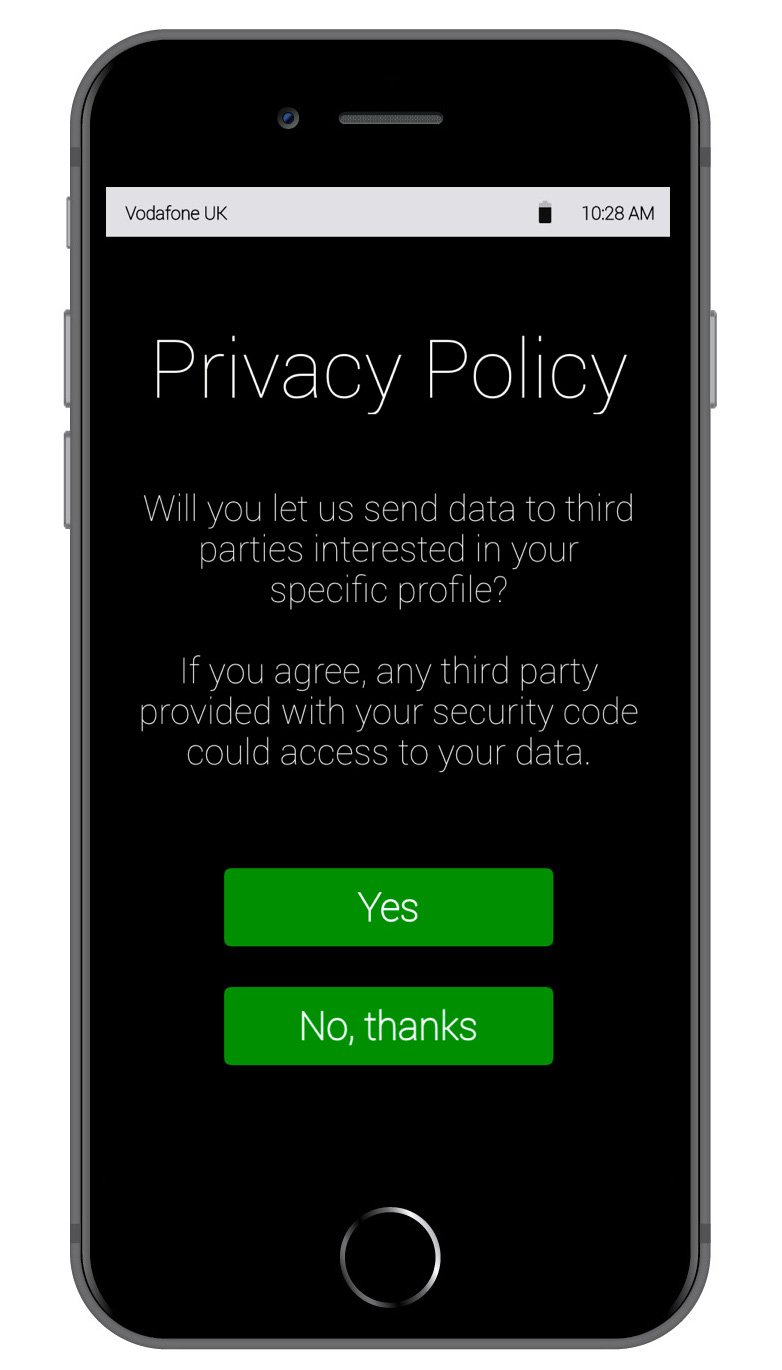
\includegraphics[height=10.4 cm]{Images/Mockups/Track4RunMockup3.jpg}
	\caption{Privacy policy conditions 2.}
        \end{minipage}%
        \hspace{10mm}%
        \begin{minipage}[c]{.40\textwidth}
        \centering
          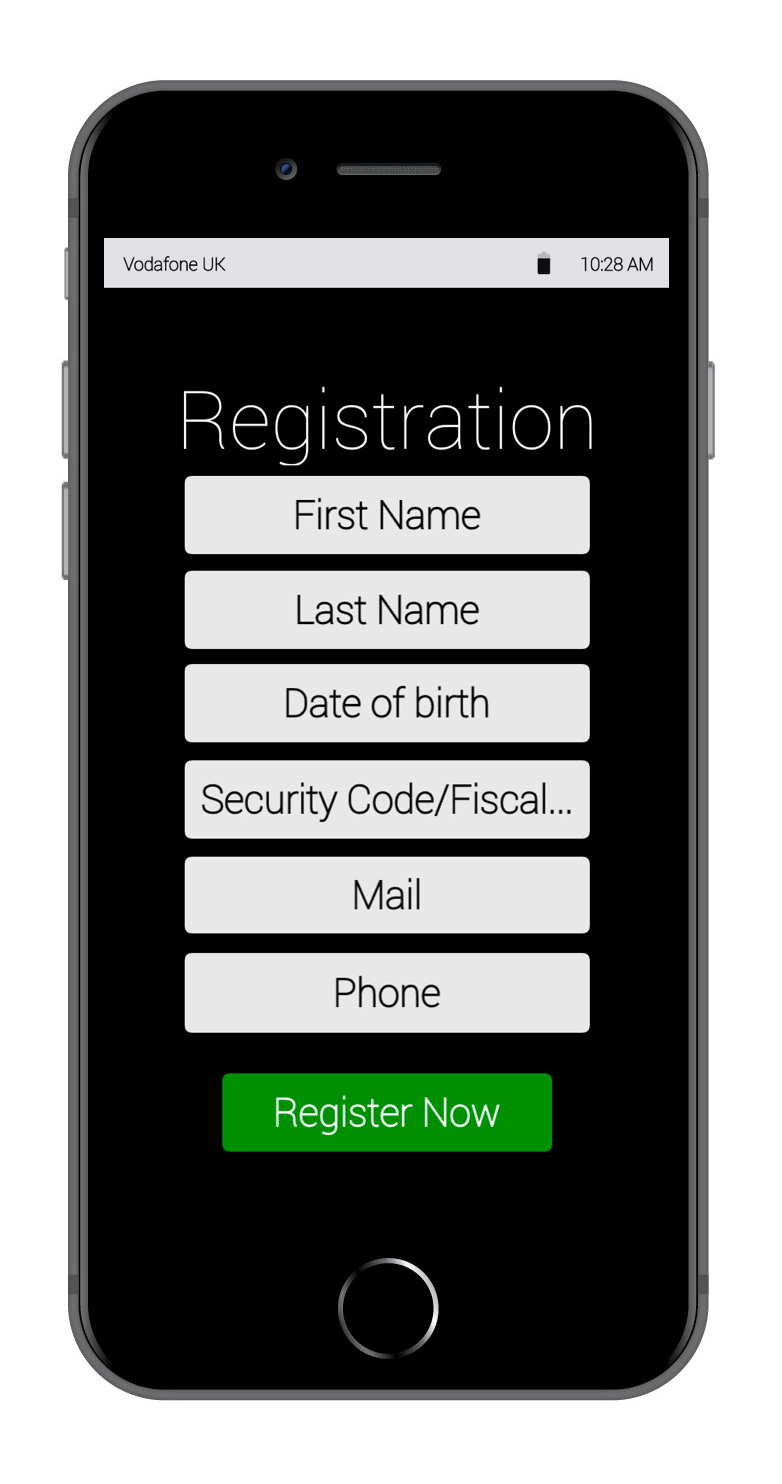
\includegraphics[height=10.4  cm]{Images/Mockups/Track4RunMockup4.jpg}
	\caption{Registration form.}
        \end{minipage}
      \end{center}
\end{figure}
\begin{figure}[H]
\begin{center}
        \begin{minipage}[c]{.40\textwidth}
        \centering
          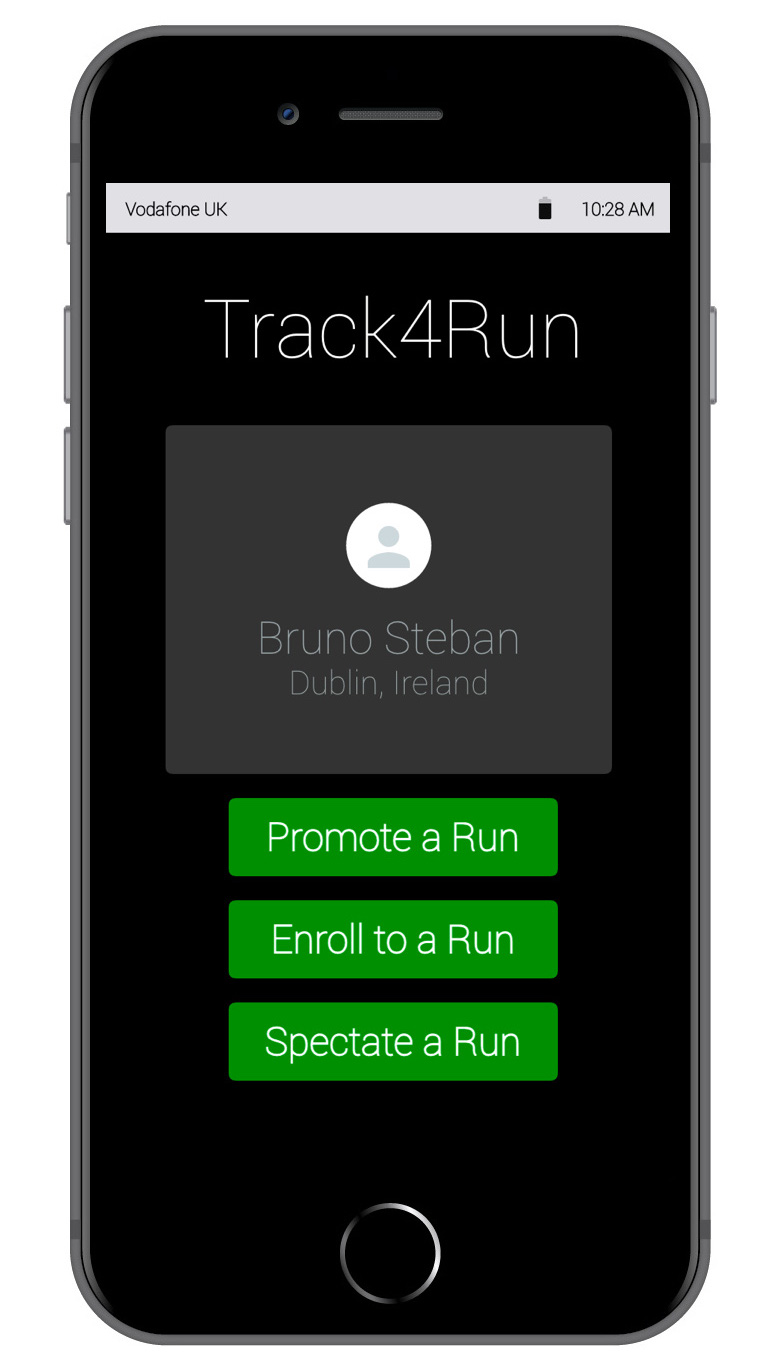
\includegraphics[height=10.4 cm]{Images/Mockups/Track4RunMockup5.jpg}
	\caption{Main user menu.}
        \end{minipage}%
        \hspace{10mm}%
        \begin{minipage}[c]{.40\textwidth}
        \centering
          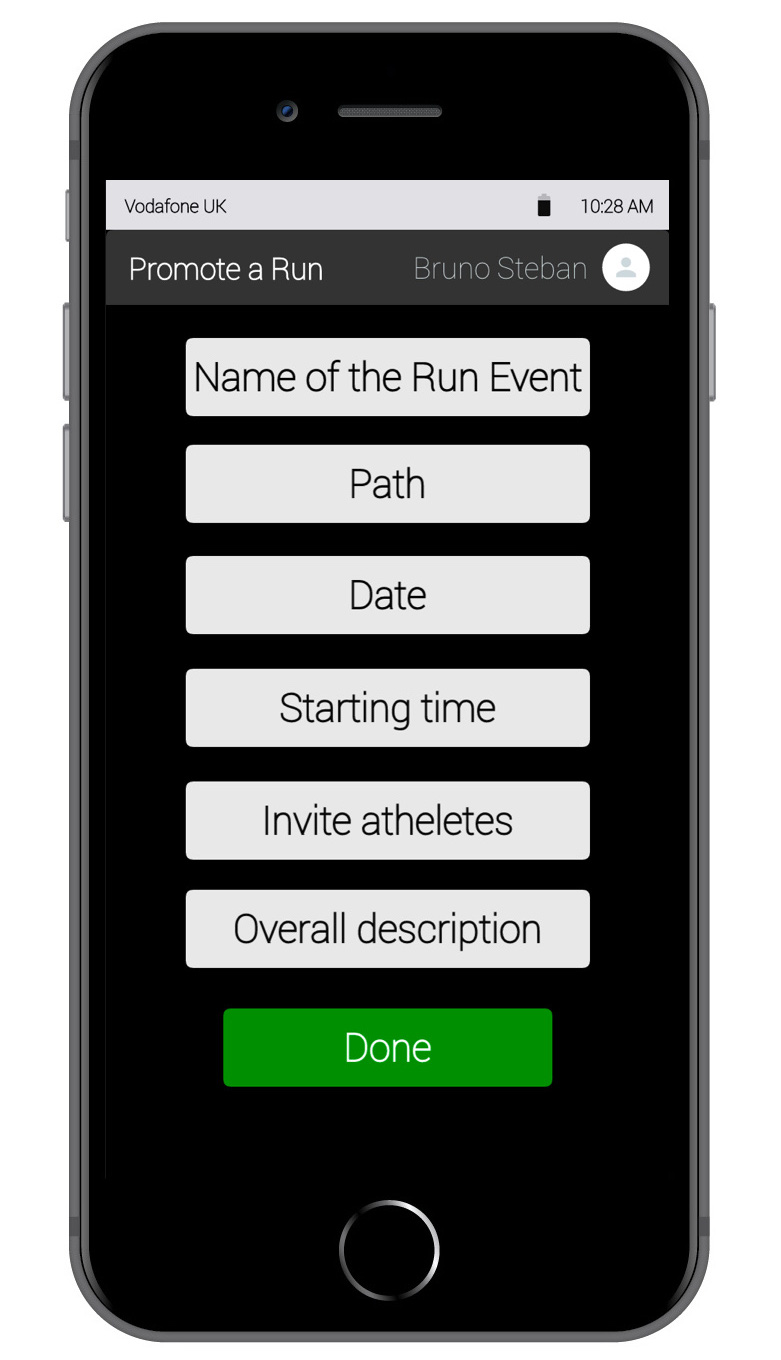
\includegraphics[height=10.4 cm]{Images/Mockups/Track4RunMockup6.jpg}
	\caption{Promote a run view.}
        \end{minipage}
      \end{center}
\end{figure}
\begin{figure}[H]
\begin{center}
        \begin{minipage}[c]{.40\textwidth}
        \centering
          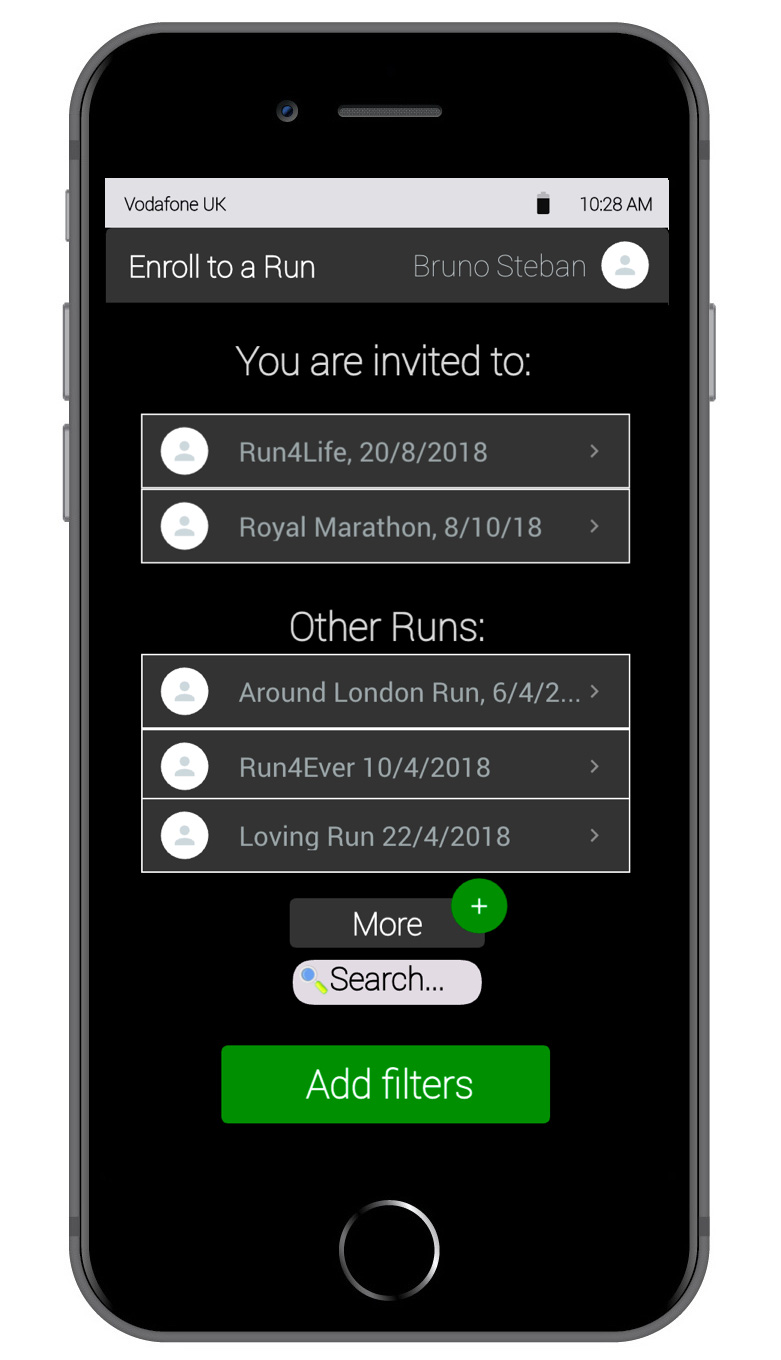
\includegraphics[height=10.4 cm]{Images/Mockups/Track4RunMockup7.jpg}
	\caption{Enroll to a run view.}
        \end{minipage}%
        \hspace{10mm}%
        \begin{minipage}[c]{.40\textwidth}
        \centering
          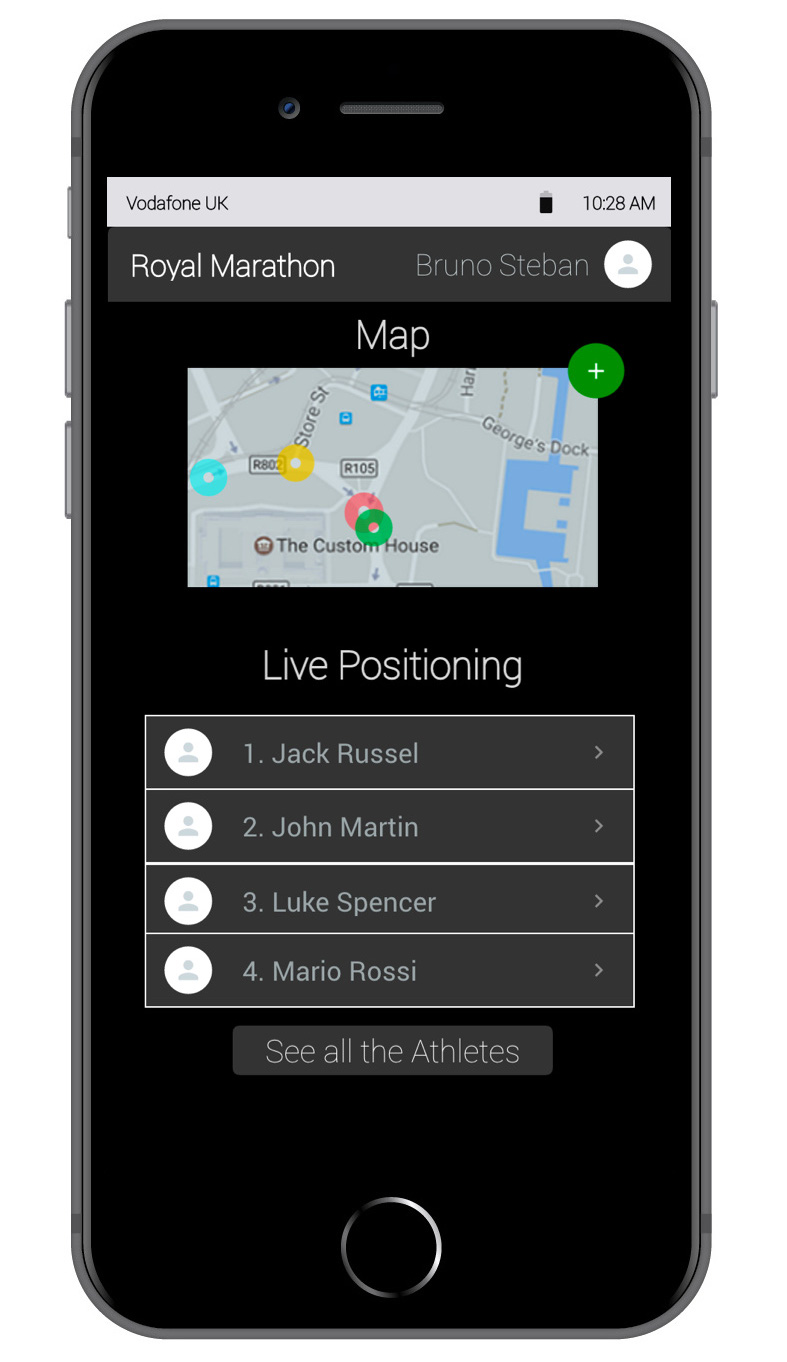
\includegraphics[height=10.4 cm]{Images/Mockups/Track4RunMockup8.jpg}
	\caption{Spectate a run view.}
        \end{minipage}
      \end{center}
\end{figure}
\end{enumerate}

\subsubsection{Hardware, Software and Communication Interfaces}
None of the three services-to-be offer any hardware or software interface to the external world. In order to send an ambulance request to the nearest hospital, AutomatedSOS uses a platform provided by the hospital. All the user data needed for the ambulance intervention (such as the location, health status and so on) are sent, for example, by email. For this reason none of the three services under analysis offer any communication interface.

\subsection{Scenarios}
\begin{enumerate}
\item[•]{\Large Scenario 1} \\
The company StatisticsDispenser is interested into weekly providing public statistics about people living in London. For this reason the company, which is already registered to Data4Help, need to send a group monitoring request. After logging into the Data4Help website, StatisticsDispenser open the group request section. The website loads a new page where the company can filter groups through some attributes regarding his members like the age, the gender, the city and many more. For the specific purpose StatisticsDispenser chooses only to filter people who live in London and people who's age is between 20 and 60. Then, due to the fact that the company need future data, StatisticsDispenser subscribes to the group. From now on every time new data is available the system sends a notification to StatisticsDispencer. 
\item[•]{\Large Scenario 2} \\
Mark often goes for a run so he decides to download an app to track his progress. The app he installed on his smartphone is a Partner Application with Data4Help. After he registers to this app he's asked if he wants to give his information to the company TrackMe and also if he wants his data to be treated also as individual data. Right after he accepts the policy he's asked to create a Data4Help account or to link an existing one to the application. Mark never created a Data4Help account so he decides to go through the registration process. He fills all the attributes fields required for the sign up and confirm the registration. Data4Help creates the account and saves all the attributes that Mark filled in. Data4Help is now ready to receive Mark's data from the partner application.
\item[•]{\Large Scenario 3} \\
Bob is 77 years old and lately he's having heart problems. Under his son's advice he decided to use the AutomatedSOS application to receive immediate aid in case of need. One month later Bob doesn't feel okay and his heartbeat value goes below the threshold. AutomatedSOS recognizes that Bob is in a critical health state and quickly sends a report to First Aid system containing useful information like his current location and the reason he's in danger. After the First Aid system received the report, it immediately sends an ambulance to Bob's location and then sends an acknowledge message to AutomatedSOS. The application shows a message on Bob's device to let him know that an ambulance is coming for aid.
\item[•]{\Large Scenario 4} \\
Mario promotes run events for a living so in order to simplify the process he goes through everyday he decides to download Track4Run on his smartphone. The famous company AdiDas designate Mario to promote a run that takes place once a year in Milan. Mario log into the app and enter the "Promote a Run" section, inserts and confirms all the information needed. Track4Run creates the run and makes it available to athletes to enroll in.
\item[•]{\Large Scenario 5} \\
Lately Eddie and his friends are bored of what they usually do so they decided to participate to a different activity. More precisely they want to create a run event using Track4Run App and see who's the fastest at running. Unfortunately Eddie got ill the day before the event but he's just too curios of seeing who of his friends is going to win. For this reason as soon as the run starts he logs into Track4Run and enters the "Spectate a Run" section and select the run created with his friends. A few moments later the map appears on the app with all the athletes positions on it letting Eddie see how the run is proceeding in real time.

\end{enumerate}

\subsection{Functional Requirements}
\begin{enumerate}
\item[•]{\Large Data4Help}
	\begin{enumerate}
	\item [G.1] \textbf{Acquire user's position and health status.}
		\begin{enumerate}
		\item [D.1] User's information are collected from partner applications or from the other two TrackMe applications installed on users' devices.
		\item [D.2] All the partner applications require to submit user credentials.
		\item [D.3] The identification (fiscal code, social security number) and the secondary data (attributes) given by the individual during the registration are correct.
		\item [R.1] Retrieve user credentials inserted into partner application as group attributes.
		\item [R.2] Allow users already registered in Data4Help world to sign in with their account without providing user credentials again.
		\item [R.3] Allow individuals to agree the privacy policy (first part) so that they can be tracked in group mode through installed application.  
		\item [R.4] During the registration allow individuals to specify if they are also interested to be tracked in single mode (agree the second part of privacy policy) through installed application. 
		\item [D.4] Devices used to monitor individuals always work and report the correct values.	
    	\item [D.5] Partner application always report correct values to Data4Help.
    	\item [R.5] For each user registered the system has to automatically retrieve and store data from partner applications with a resolution of 10 minutes; independently from the requests reached.
    	\end{enumerate}	
    	
    \item [G.2] \textbf{Provide to third parties, the user's position and health status.}
    	\begin{enumerate} 
    	\item [R.6] Allow third parties to register to Data4Help service specifying all their credentials.
		\item [R.7] The system should allow third parties to send information requests.
    	\end{enumerate}	
		
		\begin{enumerate} 
		\item [G.2.1] \textbf{Provide data on demand to non-subscribed third parties.}
		\begin{enumerate} 

		\item [R.8] The system has to collect all the useful data that match the request.
		\item [R.9] The system has to generate a statistic on data selected 
		\item [R.10] The system has to send to the third party all the raw data collected until the moment of the request.
		\item [R.11] The system has to send all the statistics already produced.
    	\end{enumerate}	
    	
    	\item [G.2.2] \textbf{Provide data in real-time to subscribed third parties.}
		\begin{enumerate}
    	\item [R.12] Allow third parties to subscribe to groups or individuals in order to receive live data.
    	\item [R.13] Provide to subscribed third parties raw data as soon as they are available by the system.
    	\end{enumerate}
    	\end{enumerate}
    
	\item [G.3] \textbf{Allow third parties two different ways to get users' data.}
		\begin{enumerate}     
    	\item [G.3.1] \textbf{Allow third parties to get data of a single person.}
		\begin{enumerate}
		\item [D.6] In order to perform an individual request, third parties has to know the user's fiscal code or security number.
		\item [D.7] Security number and fiscal code are not information given to third parties by Data4Help.
    	\item [R.14] Allow third parties to insert the fiscal code of the user he wants to track.
    	\item [R.15] Deny third parties to receive single mode information about users that have not accepted the second part of the privacy policy.
    	\item [R.8] Collect all the useful data retrieved by Data4Help that are produced by the interested users. 
    	\item [R.10] Send all the collected information to request applicant.
    	\end{enumerate}
    
    	\item [G.3.2] \textbf{Allow third parties to get data of a group of people.}
		\begin{enumerate}
    	\item [R.16] Allow third parties to insert search area and attributes in which they are interested to restrict their field of search.
    	\item [R.17] Deny third parties to receive information if the provided information can hurt users' privacy, for this purpose group request under 1000 users involved are rejected.
    	\item [R.8] Collect all the useful data retrieved by Data4Help that are produced by the interested users.
    	\item [R.10] Send all the collected information to request applicant.
    	\end{enumerate}
    	\end{enumerate}
    	
    \item [G.4] \textbf{Provide data in an anonymous way, to protect users' privacy.}
		\begin{enumerate}
    	\item [R.15] Deny third parties to receive single mode information about users that have not accepted the second part of the privacy policy.
    	\item [R.17] Deny third parties to receive information if the provided information can hurt users' privacy, for this purpose group request under 1000 users involved are rejected.
    	\end{enumerate}	
			
	\end{enumerate}
	
	
\item[•]{\Large AutomatedSOS}
	
	\begin{enumerate}
	\item [G.5] \textbf{Retrieve user's position and health status.}
		\begin{enumerate}
		\item [R.18] Allow users to be tracked from AutomatedSOS filling up the registration and agreeing only to first part of privacy policy.
		\item [D.4] Devices used to monitor individuals always report correct values.
		\item [D.9] The user always dresses a smartwatch on which AutomatedSOS is installed and running.    
		\item [R.19] The application has to retrieve users' health status every 2 seconds in order to guarantee a reaction time of 5 seconds.
		\end{enumerate}
	
	
	\item [G.6] \textbf{Monitor user's health parameters.}
		\begin{enumerate}
		\item [R.19] The application has to retrieve users' health status every 2 seconds in order to guarantee a reaction time of 5 seconds.
		\item [R.20] The application sends to Data4Help service all the data retrieved in live acquisition.
		\item [R.21] The application gets from Data4Help service all the historical data about the user.
		\item [R.22] Allow the user to set personal threshold values.
		\end{enumerate}
		
	\item [G.7] \textbf{Send an ambulance to user's location whenever certain parameters are below the threshold.}
		\begin{enumerate}
		\item [R.23] The application has to control health status with data retrieved in local to immediately realize whether certain parameters are critical.
		\item [R.24] The application sends an ambulance request to the nearest hospital whenever parameters are critical.
		\item [D.10] The first aid system is always up and ready to receive messages from AutomatedSOS.
		\item [R.25] Supply to the hospital the user's location and all the useful information to provide efficient first aid.
		\item [R.26] In the case no answer arrives from the hospital the software must repeat another time the request until an answer in reached.
		\item [R.27] As soon as the acknowledgement message is received a warning message is displayed on the user's smartwatch.
		\item [D.11] The ambulance successfully reach the location of the individual.
		\end{enumerate}
  	\end{enumerate}
  	
  	
\item[•]{\Large Track4Run}
	
	\begin{enumerate}
	\item [G.5] \textbf{Retrieve user's position and health status.}
		\begin{enumerate}
		\item [R.3] Allow individuals to agree the privacy policy (first part) so that they can be tracked in group mode through installed application.  
		\item [R.4] During the registration allow individuals to specify if they are also interested to be tracked in single mode (agree the second part of privacy policy) through installed application. 
		\item [D.4] Devices used to monitor individuals always report correct values.
		\item [R.28] The application has to interact with Smartwatch/Smartphone APIs in order to retrieve GPS location with a resolution of 10 seconds when the user is in the run .
		\end{enumerate}
		
	\item [G.8] \textbf{Allow user to manage a run.}
		\begin{enumerate}
		\item [R.29] Allow users to create a run once all the general information are inserted.
		\item [D.4] Devices used to monitor individuals always report correct values.
			
		\item [G.8.1] \textbf{Allow promoters to define a path for the run.}
			\begin{enumerate}
			\item [R.30] Allow promoters to define a path for the run by selecting the routes inside a map.
			\item [D.14] The path defined by the organizer actually exist.
			\end{enumerate}
			
		\item [G.8.2] \textbf{Allow promoters to invite athletes to the run.}
			\begin{enumerate}
			\item [R.31] Allow promoters to send a participation request.
			\item [R.32] Allow promoters to specify maximum number of athletes that can participate.
			\end{enumerate}
	\end{enumerate}
	
	\item [G.9] \textbf{Allow athlete to enroll on a specific run.}
		\begin{enumerate}
		\item [R.33] Allow the user to see all the runs generated (which he is invited or not).
		\item [R.34] Allow user to enroll in a run.
		\item [R.35] Deny user to enroll in a run if maximum number of participants is already reached.
		\item [D.16] If an athlete enroll to a run then athlete also participates to the run.
		\end{enumerate}
	
	\item [G.10] \textbf{Allow spectators to watch in real time the position of every athletes in a specific run.}
		\begin{enumerate}
		\item [R.33] Allow the user to see all the runs generated (which he is invited or not).
		\item [D.17] All athletes have their tracking devices with them and the application is enabled for the entire duration of the run.	
		\item [R.36] Allow user to select a run to be viewed.
		\item [R.37] The application requests to Data4Help the position of all the other athletes involved.
		\item [R.38] The application receives and displays the position of all the other athletes involved.
		\item [D.18] Athletes never go out of the defined path.
		\item [D.13] During a run athletes always wear a smartwatch on which Track4Run is installed.
		\end{enumerate}
	\end{enumerate}

\end{enumerate}
\clearpage

\subsubsection{Use Case Diagram}
\begin{enumerate}
\begin{minipage}{\textwidth}
\FloatBarrier
\item[•]{\Large Data4Help}
\\[2cm]
\begin{center}
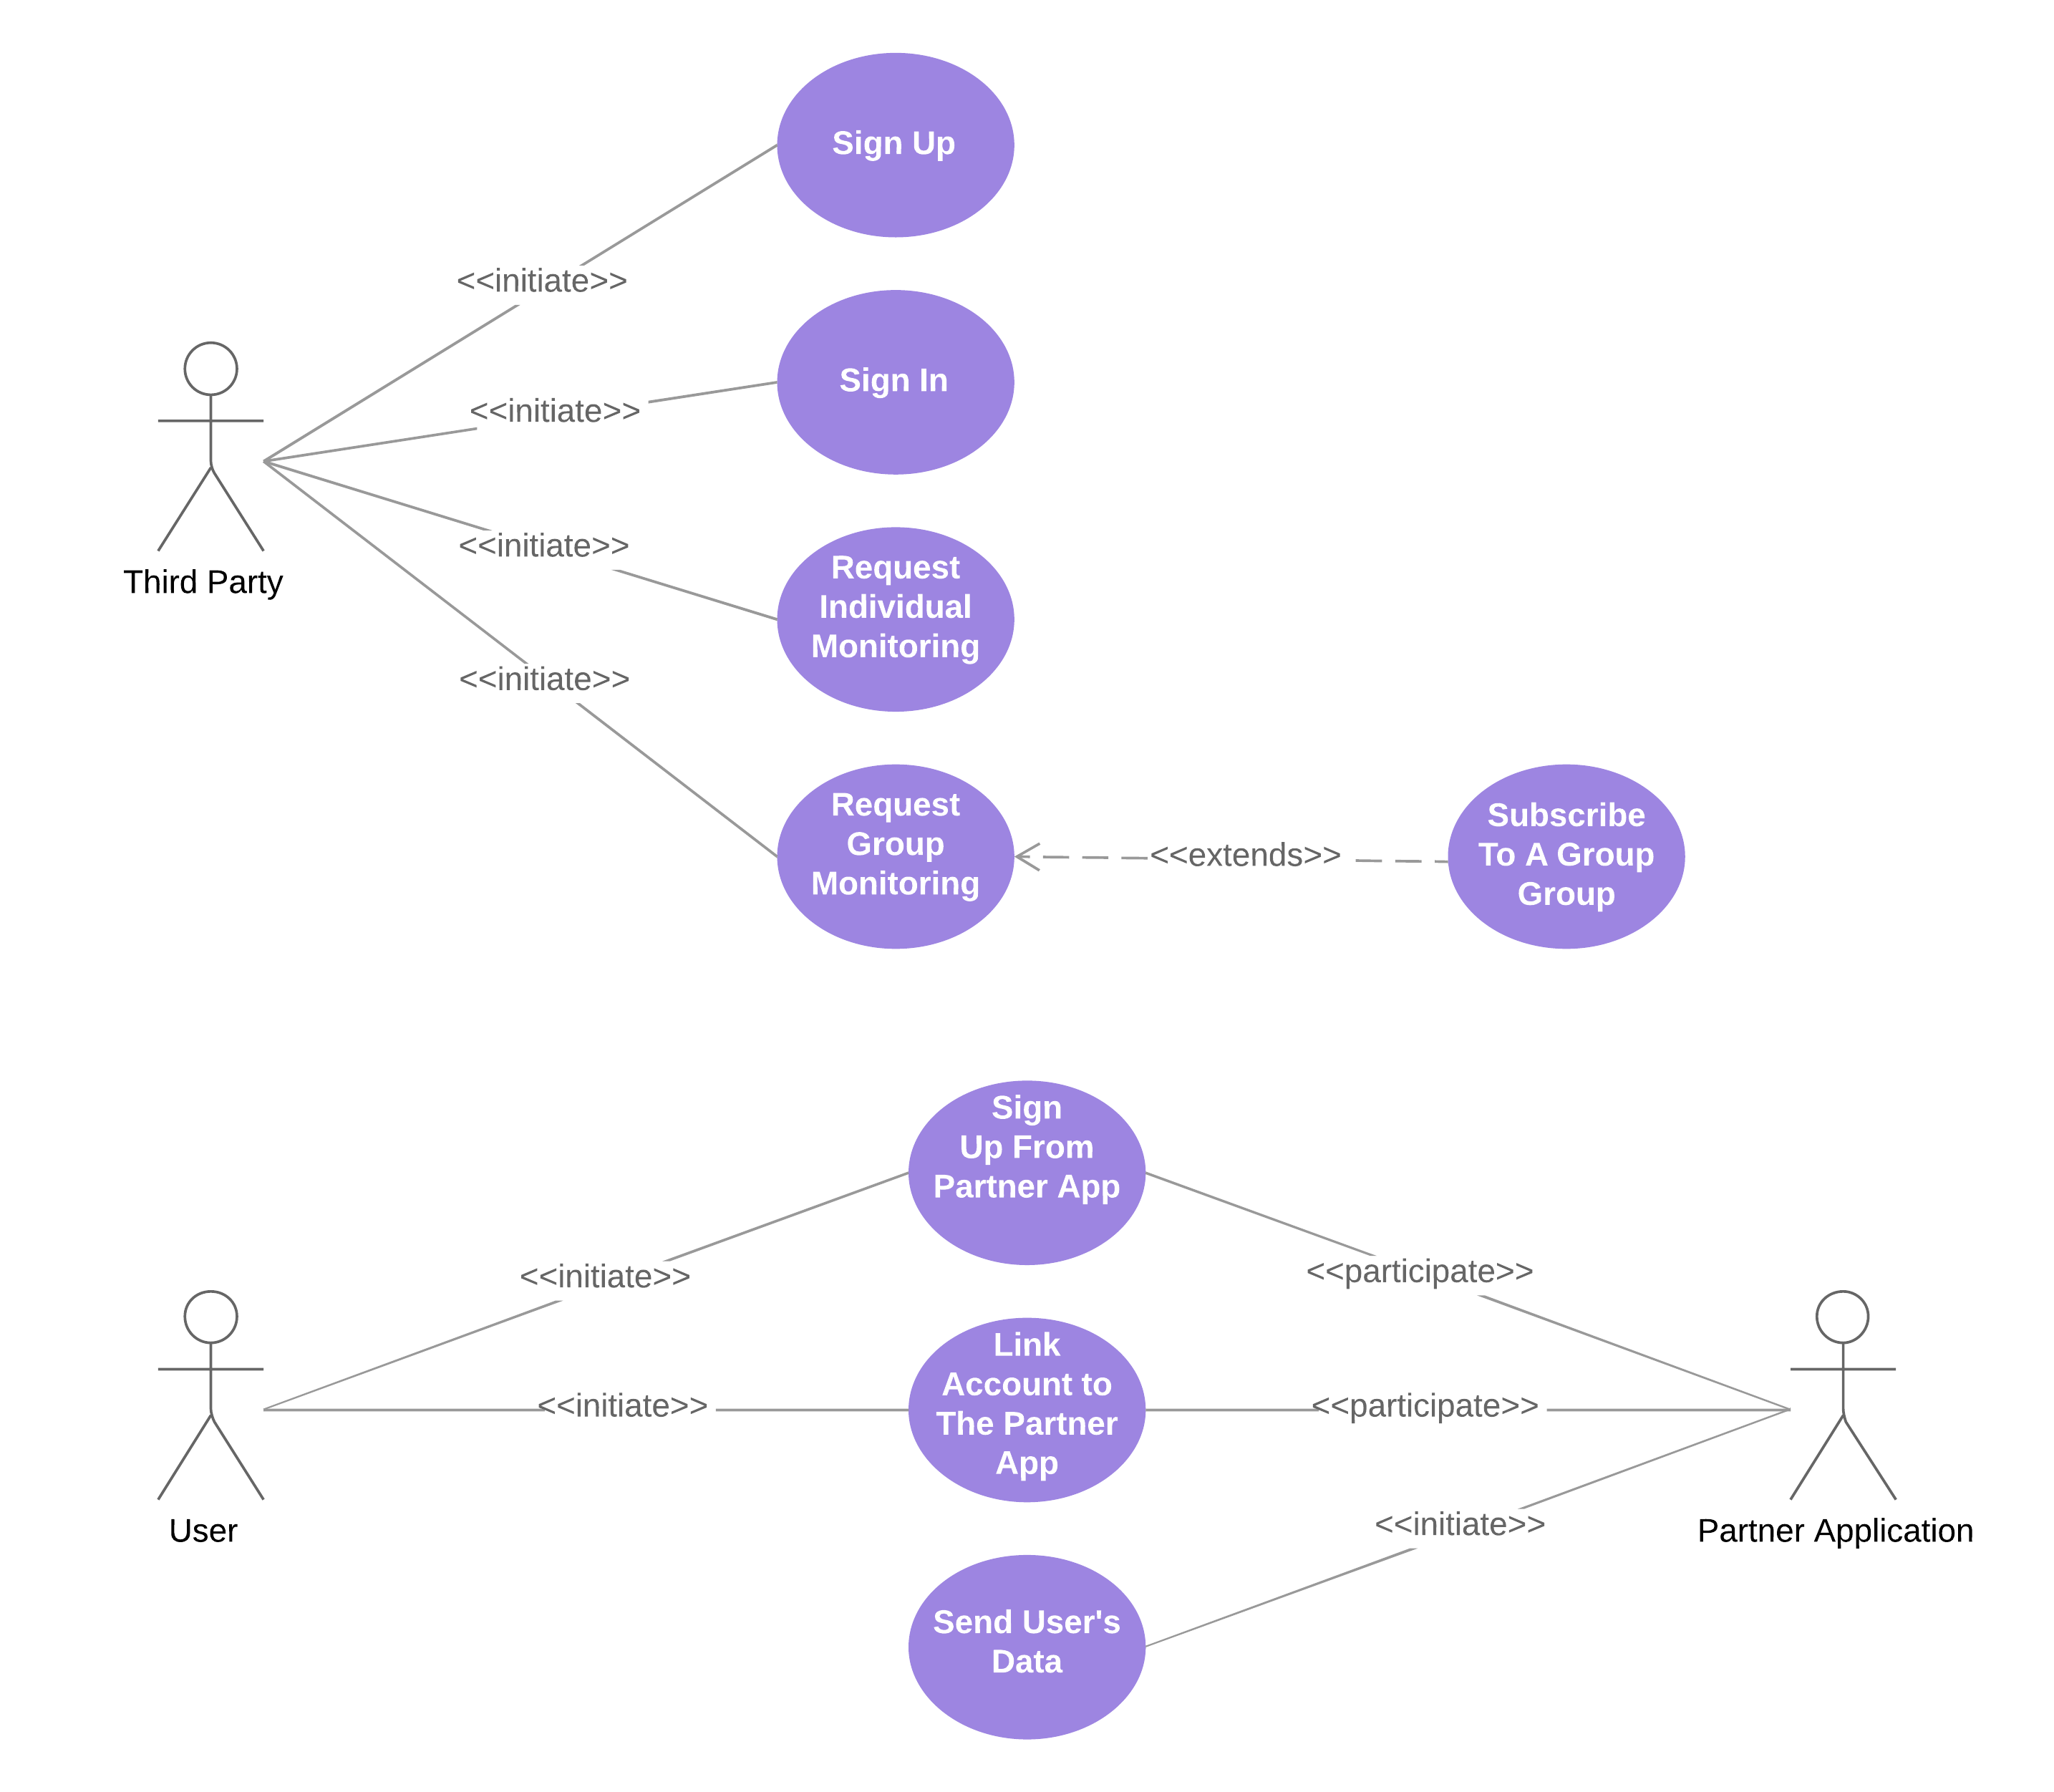
\includegraphics[scale=0.65]{Images/UseCaseDiagrams/Data4HelpUseCaseDiagram.png}
\end{center}
\FloatBarrier
\end{minipage}
\clearpage


\begin{minipage}{\textwidth}
\item[•]{\Large AutomatedSOS}
\FloatBarrier
\begin{center}
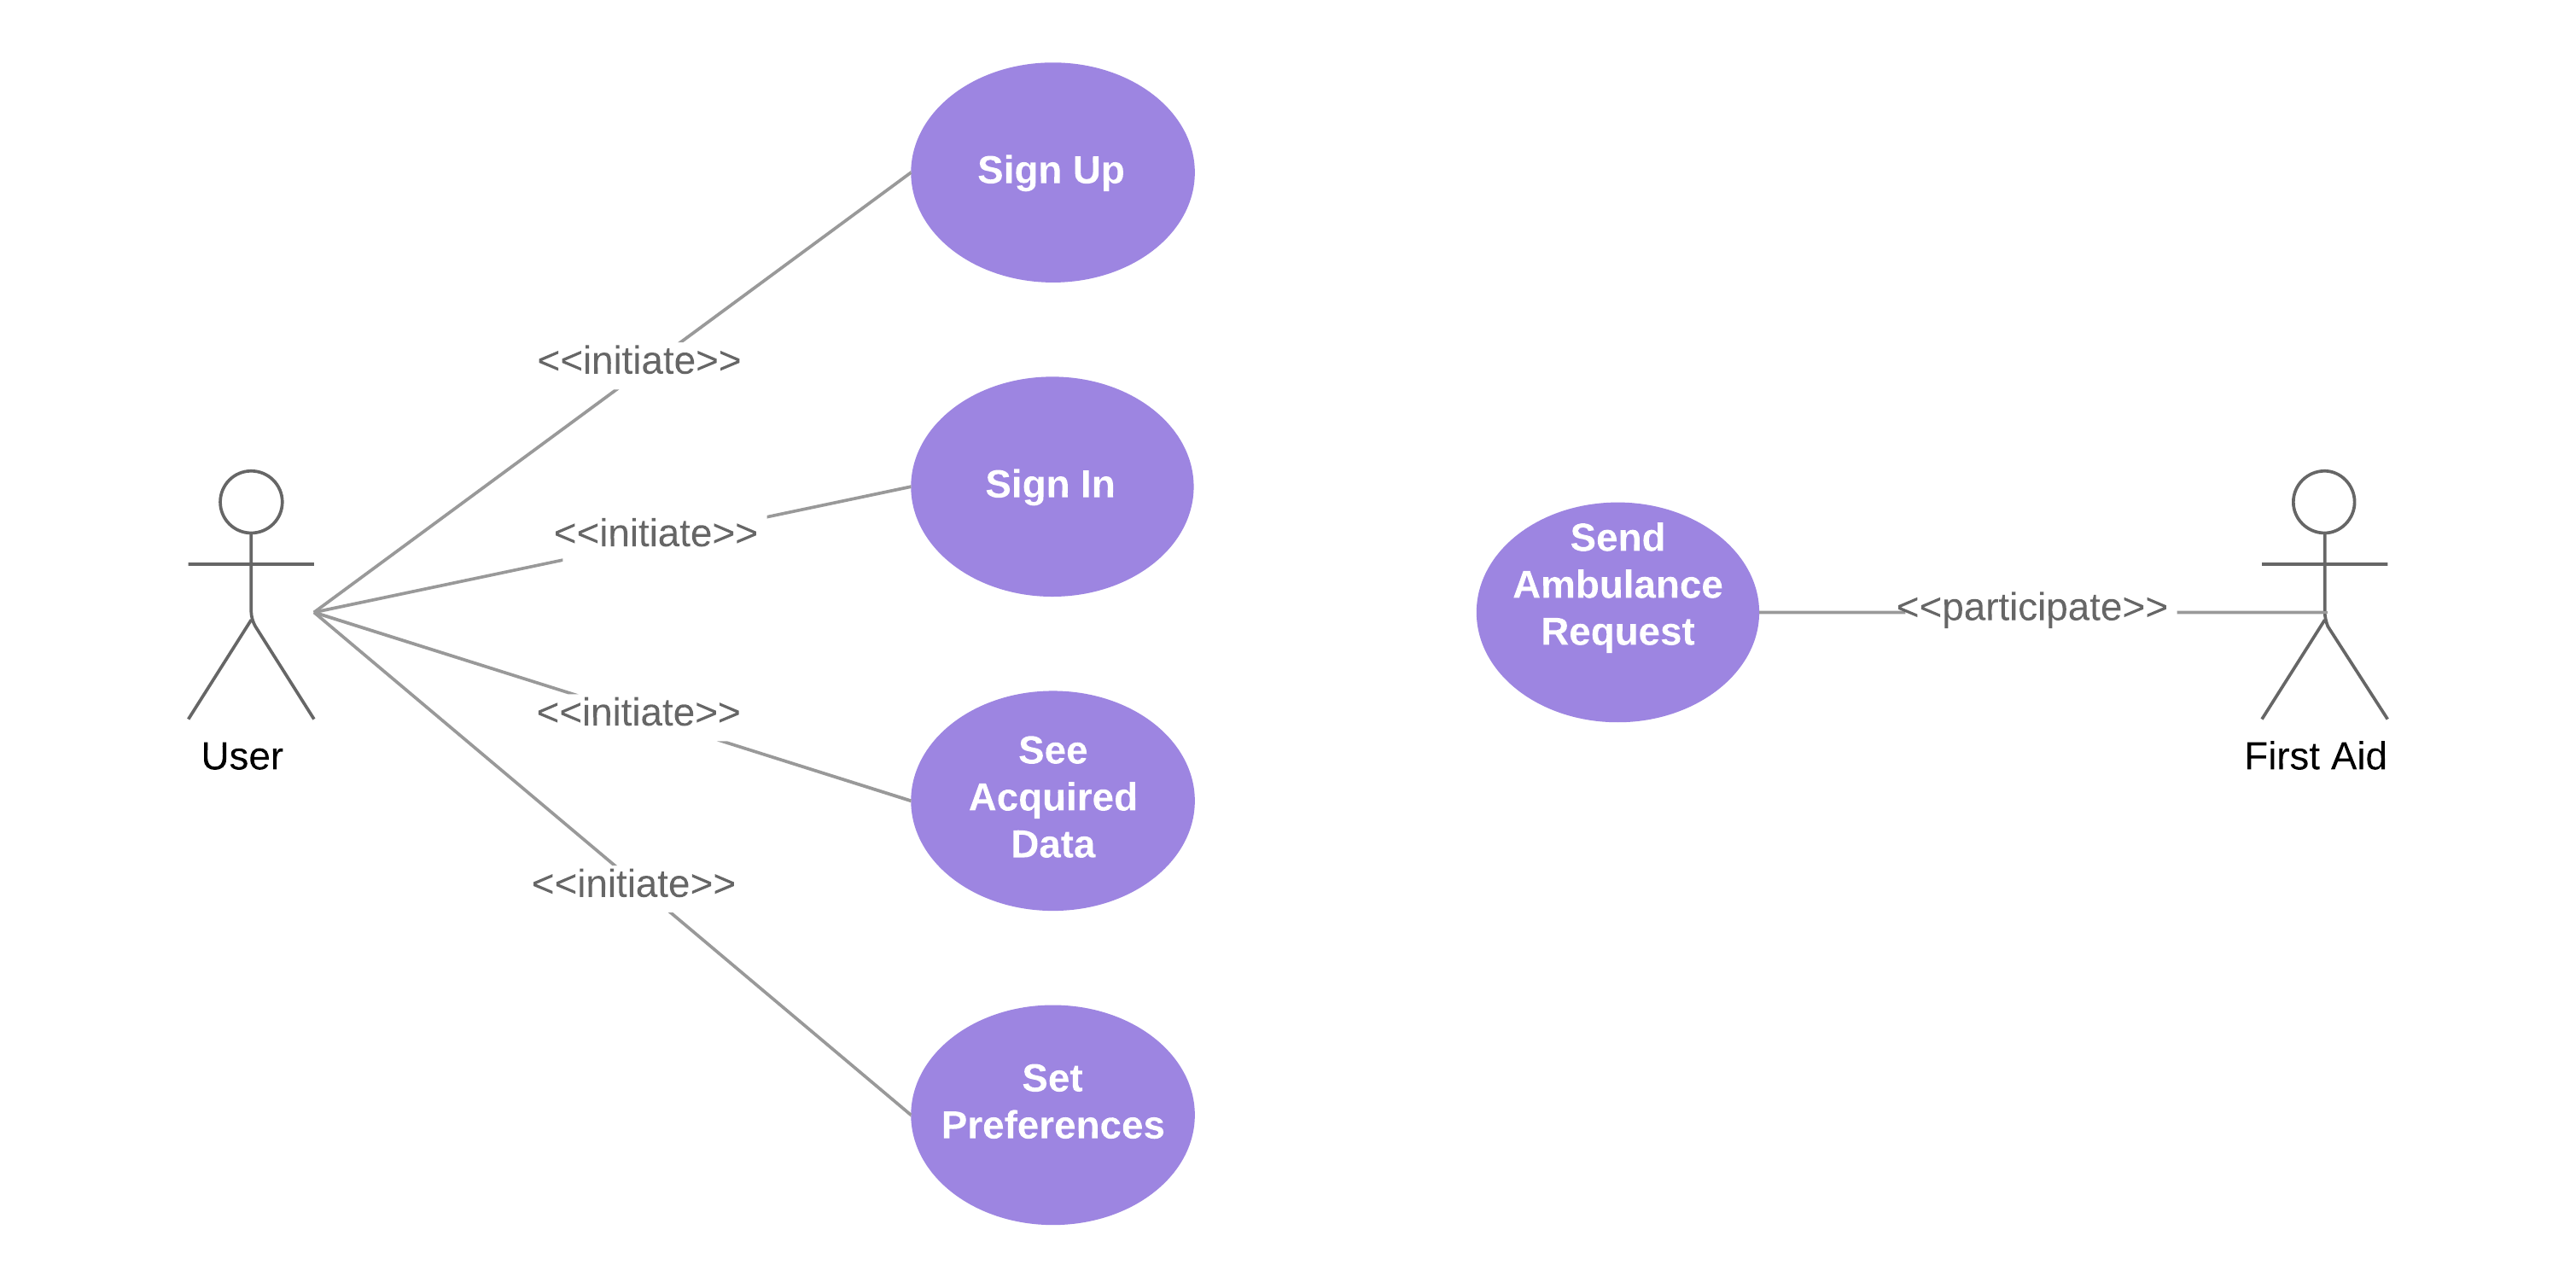
\includegraphics[scale=0.65]{Images/UseCaseDiagrams/AutomatedSOSCaseDiagram.png}
\end{center}
\FloatBarrier
\end{minipage}

\begin{minipage}{\textwidth}
\item[•]{\Large Track4Run}
\FloatBarrier
\begin{center}
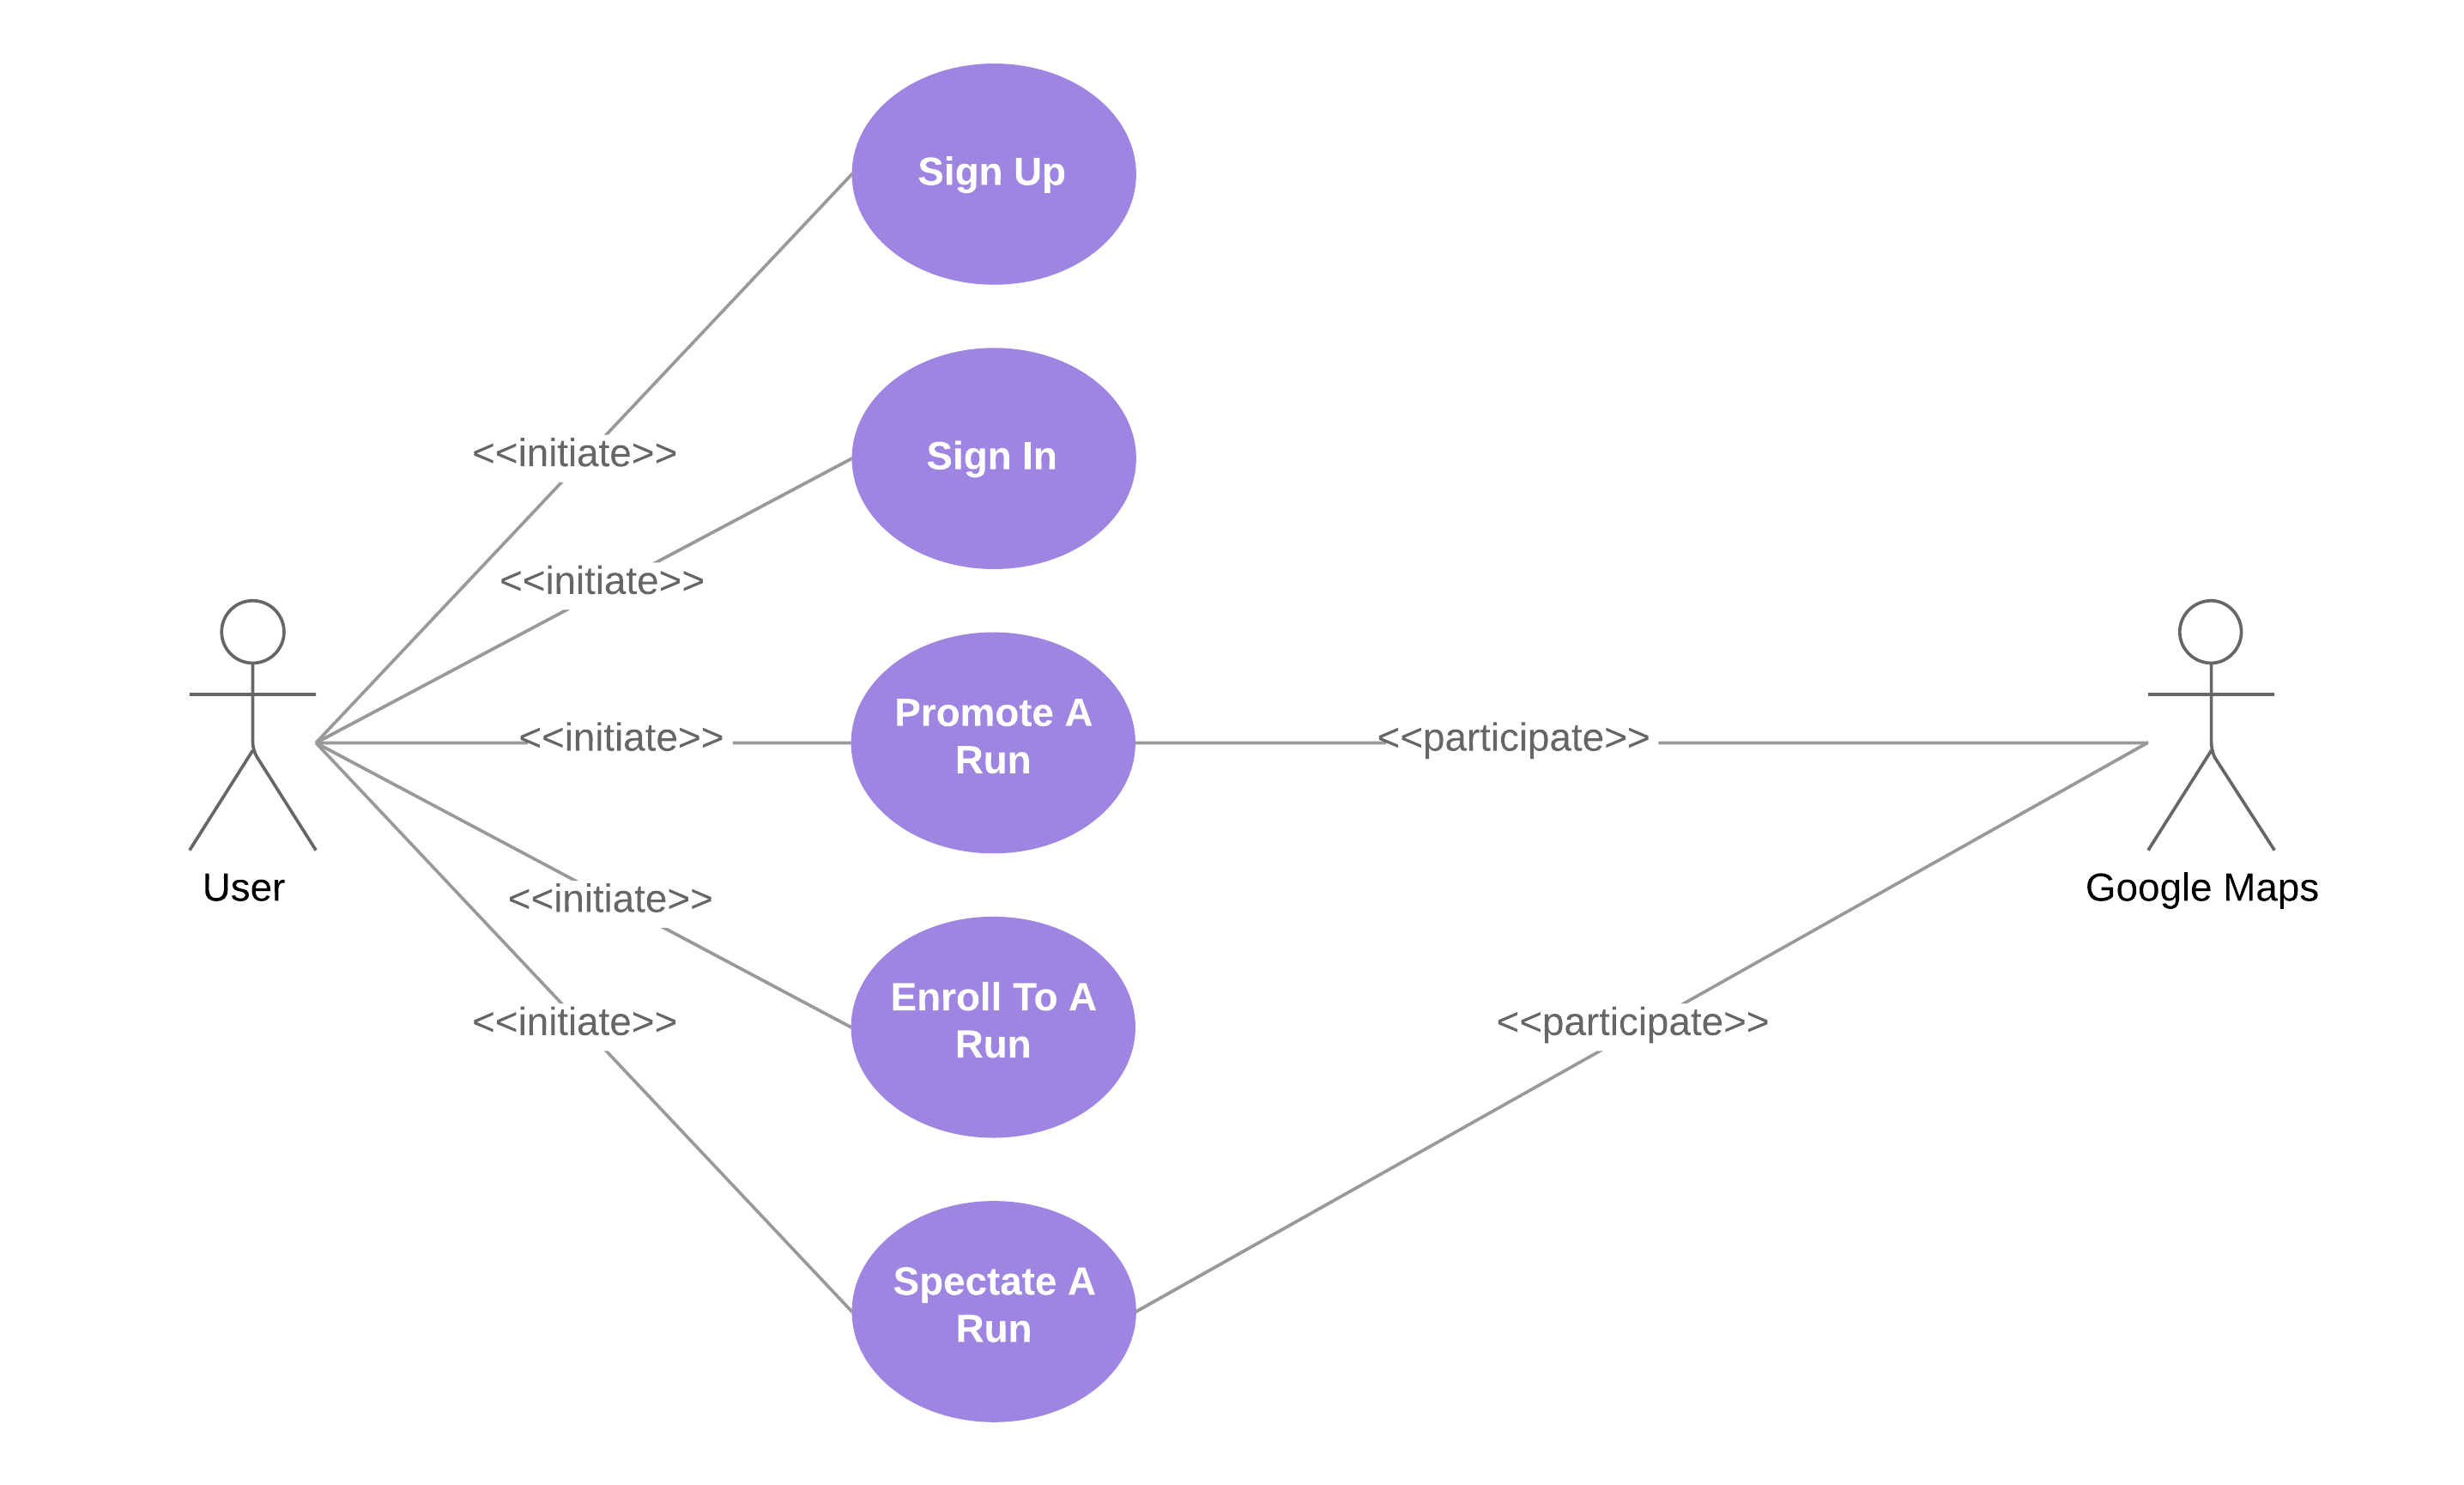
\includegraphics[scale=0.70]{Images/UseCaseDiagrams/Track4RunCaseDiagram.png}
\end{center}
\FloatBarrier
\end{minipage}
\end{enumerate}
\clearpage 

\subsubsection{Use Cases}
\begin{enumerate}
\FloatBarrier
\item[•]{\Large Data4Help Use Cases}
\FloatBarrier
\begin{table}[h]
\begin{tabular}{|l|p{.75\textwidth}|}
\hline
Name             & Sign Up \\ \hline
Actors           & Third Party \\ \hline
Entry Conditions & TRUE    \\ \hline
Event Flow       & \begin{enumerate}
            \item The Third Party enters the sign up section.
            \item The system shows to the third party all the attributes fields needed for the registration.
            \item The Third Party fills all the attribute fields.
            \item The Third Party confirms all the attributes inserted stating he wants to register.
            \item The system creates and saves the third party's account.
        \end{enumerate}\\ \hline
Exit Condition   & The third party's account has been created and the third party is now registered.\\ \hline
Exceptions       & \begin{itemize}
\item If the system notices that the attributes used in the registration are already linked to an existing account then a warning is generated saying that there is already a third party registered with the given attributes.
\end{itemize}\\ \hline
\end{tabular}
\end{table}
\FloatBarrier

\FloatBarrier
\begin{table}[h]
\begin{tabular}{|l|p{.75\textwidth}|}
\hline
Name             & Sign In \\ \hline
Actors           & Third Party  \\ \hline
Entry Conditions & TRUE   \\ \hline
Event Flow       & \begin{enumerate}
            \item The Third Party enters the sign in section.
            \item The system shows to the third party all the credentials fields needed for the log in.
            \item The Third Party fills all credentials fields and confirms he wants to log in.
            \item The system accepts the log in request.
        \end{enumerate}\\ \hline
Exit Condition   & The third party is now logged in.\\ \hline
Exceptions       & \begin{itemize}
\item If the third party inserts invalid log in credentials a warning is generated saying the credentials are invalid.
\end{itemize}\\ \hline
\end{tabular}
\end{table}
\FloatBarrier

\FloatBarrier
\begin{table}[h]
\begin{tabular}{|l|p{.75\textwidth}|}
\hline
Name             & Request Individual Monitoring and subscription\\ \hline
Actors           & Third Party  \\ \hline
Entry Conditions & The third party is logged in.    \\ \hline
Event Flow       & \begin{enumerate}
            \item The Third Party enters the Individual Request section.         
            \item The system shows to the third party all the information fields needed for the identification of the individual.
            \item The Third Party can ask to subscribe to new data as soon as they are produced (live acquisition).
            \item The Third Party fills all the attribute fields and confirms he wants to track that specific individual.
            \item The system shows all the individual's data that have been collected until the moment of the request along with some statistics. 
            \item The system subscribe the Third Party to the group if it was asked. 
        \end{enumerate}\\ \hline
Exit Condition   & The request's outcome is shown and third party is subscribed if it was asked.\\ \hline
Exceptions       & \begin{itemize}
\item If the inserted attributes are not linked to any user account then a warning message is displayed saying that the individual is not registered.
\item If the individual that correspond to the attributes inserted didn't accept the individual treatment of data policy then a warning message is displayed saying that the request is rejected.
\end{itemize}\\ \hline
\end{tabular}
\end{table}
\FloatBarrier

\FloatBarrier
\begin{table}[h]
\begin{tabular}{|l|p{.75\textwidth}|}
\hline
Name             & Request Group Monitoring and subscription \\ \hline
Actors           & Third Party  \\ \hline
Entry Conditions & The third party is logged in.    \\ \hline
Event Flow       & \begin{enumerate}
            \item The Third Party enters the Group Request section.
            \item The system shows to the third party all the information fields needed for defining the group.
            \item The Third Party insert the search area.
            \item The Third Party inserts all the attributes.
            \item The Third Party can ask to subscribe to new data as soon as they are produced (live acquisition).
            \item The system accepts the request.
            \item The system shows all the group's data that have been collected until the moment of the request along with some statistics. 
            \item The system subscribe the Third Party to the group if it was asked. 
        \end{enumerate}\\ \hline
Exit Condition   & The request's outcome is shown and third party is subscribed if it was asked.\\ \hline
Exceptions       & \begin{itemize}
\item If the group request get rejected by the system a warning message will be displayed saying the request is rejected.
\end{itemize}\\ \hline
Special Requirements & The system rejects group monitoring requests when the group's information can compromise users' privacy. For this purpose requests of groups composed by less than 1000 users get rejected.
\\ \hline
\end{tabular}
\end{table}
\FloatBarrier
\clearpage


\FloatBarrier
\begin{table}[h]
\begin{tabular}{|l|p{.75\textwidth}|}
\hline
Name             & Sign Up From Partner App\\ \hline
Actors           & User, Partner Application  \\ \hline
Entry Conditions & The user accepted the treatment of data policy.  \\ \hline
Event Flow       & \begin{enumerate}
			\item The user starts the sign up function on the partner app.
			\item The Partner Application shows to the user all the attributes fields needed for the registration.
            \item The User fills all the attribute fields.
            \item The Partner Application sends to the system the attributes inserted by the user.
            \item The system receives by the partner application all the attributes inserted by the user.
            \item The system creates the user's account and saves the received data.
        \end{enumerate}\\ \hline
Exit Condition   & The system registered the user.\\ \hline
Exceptions       & \begin{itemize}
\item If the system notices that attributes used in the registration are already linked to an existing account then a message is sent back to the partner application in order to let the user know what happened.
\end{itemize}\\ \hline
\end{tabular}
\end{table}
\FloatBarrier

\FloatBarrier
\begin{table}[h]
\begin{tabular}{|l|p{.75\textwidth}|}
\hline
Name             & Link Account To The Partner App\\ \hline
Actors           & User, Partner Application  \\ \hline
Entry Conditions & The user accepted the treatment of data policy and already has an existing account to link to the partner application.  \\ \hline
Event Flow       & \begin{enumerate}
			\item The user starts the account linking function on the partner app.
			\item The Partner Application shows to the user all the credential fields needed for the linking process.
            \item The User fills all the credential fields.
            \item The Partner Application sends to the system the credentials inserted by the user.
            \item The system receives by the partner application all the credentials inserted by the user.
            \item The system sends back to the partner application the outcome of the operation. 
        \end{enumerate}\\ \hline
Exit Condition   & The system registered the user.\\ \hline
Exceptions       & \begin{itemize}
\item If the system notices that the credentials received are not linked to an existing account then a message is sent back to the partner application in order to let the user know what happened.
\end{itemize}\\ \hline
\end{tabular}
\end{table}
\FloatBarrier


\FloatBarrier
\begin{table}[h]
\begin{tabular}{|l|p{.75\textwidth}|}
\hline
Name             & Send User's Data\\ \hline
Actors           & User, Partner Application  \\ \hline
Entry Conditions & The user accepted the treatment of data policy and the partner application is running on the user's device.  \\ \hline
Event Flow       & \begin{enumerate}
			\item The Partner Application collects user's data.
            \item The Partner Application sends the user's data to the the system.
            \item The system receives and saves the user's data sent by the partner application.
        \end{enumerate}\\ \hline
Exit Condition   & The system saved the user's data.\\ \hline
Exceptions       & None \\ \hline
\end{tabular}
\end{table}
\FloatBarrier
\newpage

\item[•]{\Large AutomatedSOS Use Cases}
\FloatBarrier
\begin{table}[h]
\begin{tabular}{|l|p{.75\textwidth}|}
\hline
Name             & Sign Up \\ \hline
Actors           & User  \\ \hline
Entry Conditions & The User has AutomatedSOS installed on his smartwatch.    \\ \hline
Event Flow       & \begin{enumerate}
            \item The User enters the sign up section of the app.
            \item The User accepts the treatment of data policy.
            \item The system shows to the user all the attributes fields needed for the registration.
            \item The User fills all the attribute fields.
            \item The User confirms all the attributes inserted stating he wants to register.
            \item The system creates and saves the user's account.
        \end{enumerate}\\ \hline
Exit Condition   & The user's account has been created and the user is now registered.\\ \hline
Exceptions       & \begin{itemize}
\item If the User does not accept the treatment of data policy then a warning is generated saying that ,in order to register, the policy must be accepted.
\item If the system notices that attributes used in the registration are already linked to an existing account then a warning is generated saying that there is already an individual registered with the given credentials.
\end{itemize}\\ \hline
\end{tabular}
\end{table}
\FloatBarrier

\FloatBarrier
\begin{table}[h]
\begin{tabular}{|l|p{.75\textwidth}|}
\hline
Name             & Sign In \\ \hline
Actors           & User  \\ \hline
Entry Conditions & The User has AutomatedSOS application installed on his smartwatch.    \\ \hline
Event Flow       & \begin{enumerate}
			\item The User enters the sign in section of the app.
            \item The system shows to the user all the credentials fields needed for the log in.
            \item The User fills all credentials fields and confirms he wants to log in.             
            \item The system accepts the log in request.
        \end{enumerate}\\ \hline
Exit Condition   & The User user is now logged in.\\ \hline
Exceptions       & \begin{itemize}
\item If the user inserts invalid log in credentials a warning is generated saying the credentials are invalid.
\end{itemize}\\ \hline
\end{tabular}
\end{table}
\FloatBarrier

\FloatBarrier
\begin{table}[h]
\begin{tabular}{|l|p{.75\textwidth}|}
\hline
Name             & See Acquired Data \\ \hline
Actors           & User  \\ \hline
Entry Conditions & The User is logged in. \\ \hline
Event Flow       & \begin{enumerate}
            \item The User enters the Acquired Info section of the app.
            \item The system gets all the user's information that have been retrieved by the application until that moment.
            \item The system displays the user's information.
\end{enumerate}\\ \hline
Exit Condition   & All the information retrieved by the system are shown on the app.\\ \hline
Exceptions       & \begin{itemize}
\item If the system do not find information about the user then a warning message is shown to the user saying that until now the application did not record any information.
\end{itemize}  \\ \hline
\end{tabular}
\end{table}
\FloatBarrier

\FloatBarrier
\begin{table}[h]
\begin{tabular}{|l|p{.75\textwidth}|}
\hline
Name             & Set Preferences \\ \hline
Actors           & User  \\ \hline
Entry Conditions & The User is logged in. \\ \hline
Event Flow       & \begin{enumerate}
            \item The User enters the Preferences section of the application.
            \item The User can add or remove certain health parameters in order to personalize the monitoring profile.
            \item The User can also change certain parameters threshold.
            \item The User confirms all the changes done.
            \item The system saves all the changes made by the user.
        \end{enumerate}\\ \hline
Exit Condition   & The parameters are correctly updated as the user wants them to be.\\ \hline
Exceptions       & \begin{itemize}
\item If the user does not confirm the changes then all parameters remain the same as before. 
\end{itemize} \\ \hline
\end{tabular}
\end{table}
\FloatBarrier

\FloatBarrier
\begin{table}[h]
\begin{tabular}{|l|p{.75\textwidth}|}
\hline
Name             & Send Ambulance Request \\ \hline
Actors           & AutomatedSOS, First Aid  \\ \hline
Entry Conditions & A critical health parameter value is below the threshold.
\\ \hline
Event Flow       & \begin{enumerate}
            \item AutomatedSOS sends to First Aid a report that contains all important information about the user like his current location, his gender, his age, his health profile, and the list of parameters that got below the threshold.
            \item First Aid immediately sends an ambulance to the user's location.
			\item First Aid sends an acknowledge message to AutomatedSOS.            
            \item AutomatedSOS displays on the app a warning message saying that an ambulance is currently heading to the user's location. 
        \end{enumerate}
\\ \hline
Exit Condition   & A warning message is shown saying that an ambulance is currently heading to the user's location.
\\ \hline
Exceptions       & \begin{itemize}
\item If no acknowledge message is received by AutomatedSOS after the form has been sent, as soon as a certain time out expires AutomatedSOS re-send the form with updated information. 
\end{itemize}
\\ \hline
Special Requirements & The form need to be sent to First Aid with a reaction time of less than 5 seconds from the time the parameters are below the threshold.
\\ \hline 
\end{tabular}
\end{table}
\FloatBarrier

\FloatBarrier
\item[•]{\Large Track4Run Use Cases}
\begin{table}[h]
\begin{tabular}{|l|p{.75\textwidth}|}
\hline
Name             & Sign Up \\ \hline
Actors           & User  \\ \hline
Entry Conditions & The User has Track4Run application installed on his device.    \\ \hline
Event Flow       & \begin{enumerate}
			\item The User enters the sign up section of the app.
            \item The User accepts the treatment of data policy.
            \item The system shows to the user all the attributes fields needed for the registration.
            \item The User fills all the attribute fields.
            \item The User confirms all the attributes inserted stating he wants to register.
            \item The system creates and saves the user's account.
        \end{enumerate}\\ \hline
Exit Condition   & The user's account has been created and the user is now registered.\\ \hline
Exceptions       & \begin{itemize}
\item If the User does not accept the treatment of data policy then a warning is generated saying that ,in order to register, the policy must be accepted.
\item If the system notices that attributes used in the registration are already linked to an existing account then a warning is generated saying that there is already an individual registered with the given credentials.
\end{itemize}\\ \hline
\end{tabular}
\end{table}
\FloatBarrier

\FloatBarrier
\begin{table}[h]
\begin{tabular}{|l|p{.75\textwidth}|}
\hline
Name             & Sign In \\ \hline
Actors           & User  \\ \hline
Entry Conditions & The User has Track4Run application installed on his smartwatch.    \\ \hline
Event Flow       & \begin{enumerate}
			\item The User enters the sign in section of the app.
            \item The system shows to the user all the credentials fields needed for the log in.
            \item The User fills all credentials fields and confirms he wants to log in.
            \item The system accepts the log in in request.
        \end{enumerate}\\ \hline
Exit Condition   & The User user is now logged in.\\ \hline
Exceptions       & \begin{itemize}
\item If the user inserts invalid log in credentials a warning is generated saying the credentials are invalid.
\end{itemize}\\ \hline
\end{tabular}
\end{table}
\FloatBarrier

\FloatBarrier
\begin{table}[h]
\begin{tabular}{|l|p{.75\textwidth}|}
\hline
Name             & Promote A Run \\ \hline
Actors           & User  \\ \hline
Entry Conditions & The User is logged in.    \\ \hline
Event Flow       & \begin{enumerate}
            \item The User enters the Promote a Run section of the app.
            \item The system shows to the user a new tab where the user can define all the important information about the run and also invite athletes.
            \item The system creates and saves the run's information.
            \item The system automatically sends notifications to all athletes specified by the promoter asking them if they want to participate to the run.
        \end{enumerate}\\ \hline
Exit Condition   & The run event has been created and added to the list of promoted runs.\\ \hline
Exceptions       & \begin{itemize}
\item If the user does not insert critical information (like the path, the name or the date) a warning message is shown saying that critical parameters are missing.
\end{itemize}\\ \hline
\end{tabular}
\end{table}
\FloatBarrier

\FloatBarrier
\begin{table}[h]
\begin{tabular}{|l|p{.75\textwidth}|}
\hline
Name             & Enroll To A Run \\ \hline
Actors           & User  \\ \hline
Entry Conditions & The User is logged in.    \\ \hline
Event Flow       & \begin{enumerate}
            \item The User enters to the "Enroll to a Run" section of the app.
            \item The system shows to the user a list containing all invites received and also a second list containing all created runs taking place in the future.
            \item The User can filter the runs with some attributes.
            \item The User chooses the run he wants to participate to.
            \item The system enrolls the user to the run.
        \end{enumerate}\\ \hline
Exit Condition   & The user is now enrolled to the chosen run.\\ \hline
Exceptions       & \begin{itemize}
\item If the chosen run has already capped the maximum amount of athletes then a warning message is displayed saying that no more athletes are allowed to participate to the run.
\end{itemize}\\ \hline
\end{tabular}
\end{table}
\FloatBarrier

\FloatBarrier
\begin{table}[h]
\begin{tabular}{|l|p{.75\textwidth}|}
\hline
Name             & Spectate A Run \\ \hline
Actors           & User  \\ \hline
Entry Conditions & The User is logged in.    \\ \hline
Event Flow       & \begin{enumerate}
            \item The User enters the Spectate a Run section of the app.
            \item The system shows a new tab where the list of all live runs is visible.
            \item The User can filter the runs with some attributes.
            \item The User chooses the run he wants to spectate.
            \item The system shows to the user the map of the run and also the position of all athletes in real time.
        \end{enumerate}\\ \hline
Exit Condition   & The system is showing to the user the map and the athletes positions.\\ \hline
Exceptions       & None.\\ \hline
\end{tabular}
\end{table}
\clearpage
\FloatBarrier

\end{enumerate}



\subsection{Sequence Diagram}
\begin{enumerate}
\begin{minipage}{\textwidth}
\FloatBarrier
\item[•]{\Large Data4Help}


Individual request with on-demand acquisition performance.
\begin{center}
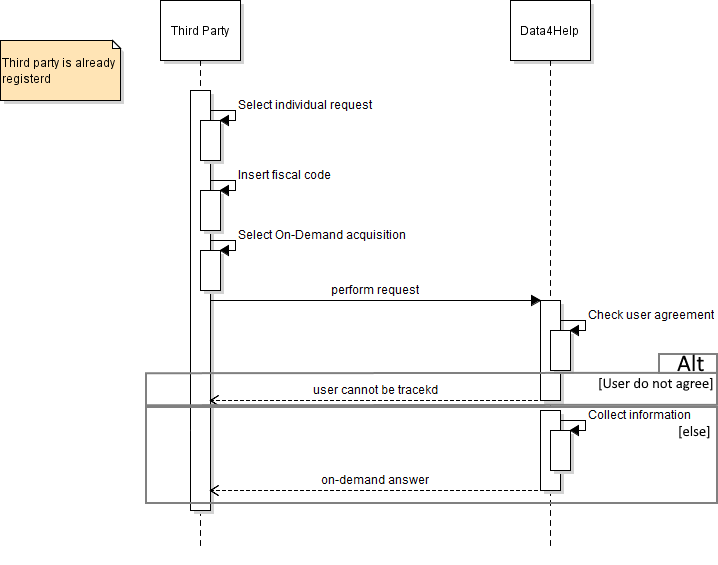
\includegraphics[scale=0.8]{Images/Seq_Data4Help_onDem.png}
\end{center}
\FloatBarrier

\FloatBarrier
Automatic data update inside Data4Help.
\begin{center}
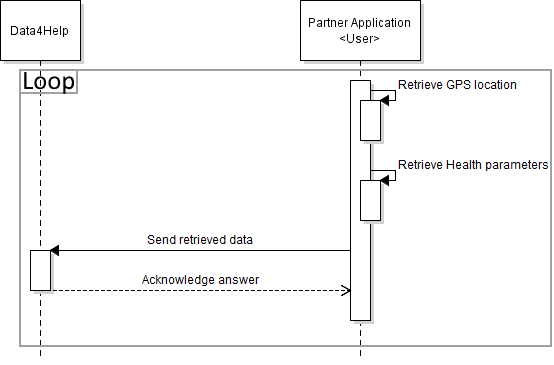
\includegraphics[scale=0.8]{Images/Seq_Data4Help_autoUp.png}
\end{center}
\FloatBarrier

\end{minipage}

\begin{minipage}{\textwidth}
\FloatBarrier
Group request with live acqusition performance.
\begin{center}
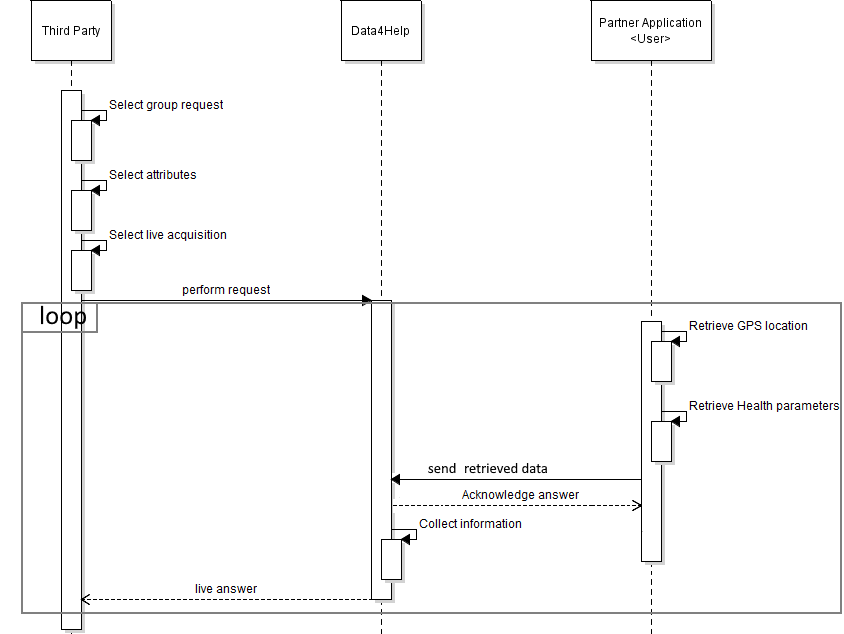
\includegraphics[scale=0.72]{Images/Seq_Data4Help_live.png}
\end{center}

\FloatBarrier
User registration performance.
\begin{center}
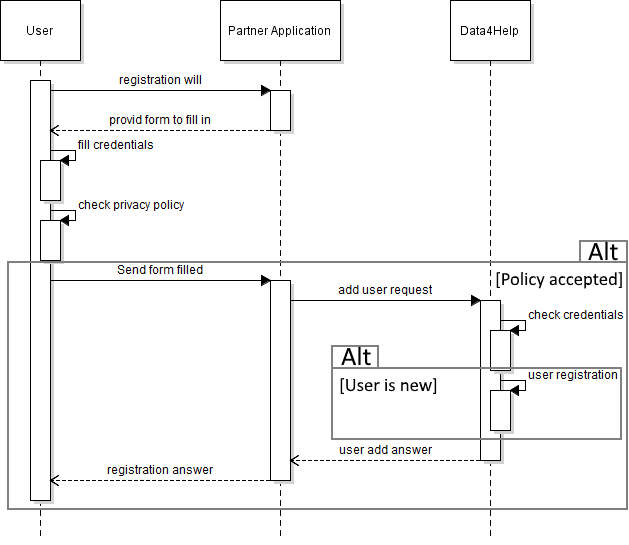
\includegraphics[scale=0.72]{Images/Seq_Data4Help_registration.png}
\end{center}


\FloatBarrier
\end{minipage}


\begin{minipage}{\textwidth}
\item[•]{\Large AutomatedSOS}
\FloatBarrier
AutomatedSOS monitor and ambulance caller services.
\begin{center}
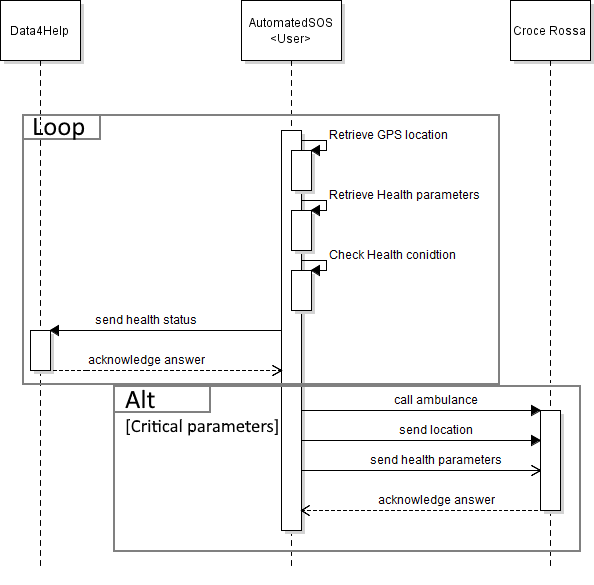
\includegraphics[scale=0.77]{Images/Seq_AutoSOS_monitor.png}
\end{center}
\FloatBarrier

\item[•]{\Large Track4Run}
\FloatBarrier
Track4Run automated retrieve athletes' position and update spectators' live map.
\begin{center}
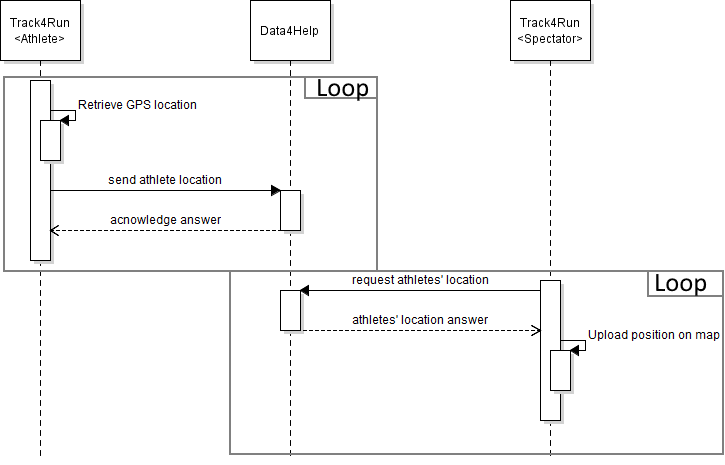
\includegraphics[scale=0.77]{Images/Seq_Track4Run_raceUp.png}
\end{center}
\FloatBarrier
\end{minipage}

\end{enumerate}


\subsection{Performance Requirements}
\begin{enumerate} 
\item[•] Data4Help service is build to perform trend research from users that download specific partner applications. In order to perform this type of monitoring there is a high use of resources, especially in live acquisition when data must be exchanged within 2 minutes. Therefore , in its first release, this application is developed to track 10.000 users simultaneously (included users from AutomateSOS and Track4Run). 
Since third parties are very few in comparison to users, to serve them a less performance is required. 

\item[•] Data4Help unsubscribes third parties after one month from live acquisition because it is a very expensive process.

\item[•] AutomatedSOS is a very expensive application in terms of performance because it must monitor the individuals all the day long guarantying a data collection with an interval of 2 seconds.

\item[•] Track4Run is a variable expensive application because it has to monitor constantly during the run events (even not all day) the athletes which are participating to them.
\end{enumerate}

\subsection{Design Constraints}
\subsubsection{Standards compliance}
\begin{enumerate} 
\item[•] Partner applications request the permission to retrieve location and health status to the device, same for AutomateSOS and Track4Run.
\item[•] Data4Help requires that partner applications can use internet connection and users' mobile data to exchange information.
\item[•] AutomatedSOS requires all day internet connection in order to call an ambulance every time is needed.
\item[•] AutomatedSOS requires internet connection during all the duration of the race to the athletes and to the spectator.
\end{enumerate}

\subsubsection{Hardware limitations}
\begin{enumerate} 
\item[•] AutomatedSOS application needs to be installed on a smartwatch (smartphone is not enough) in order to acquire location and health status.
\item[•] Track4Run application requires to be installed on a smartphone or a smartwatch in order to acquire location.
\item[•] Smartphones and smartwatches must be iOS or Android platform.
\item[•] The devices must have internet connection (mobile data are mandatory).
\item[•] The devices must have GPS locator.
\item[•] Smartwatches must have Heart Rate monitor, Blood Pressure monitor, Pedometer, Calories Calculator.
\end{enumerate}

\subsection{Software System Attributes}
\subsubsection{Reliability}
Data4Help service,clearly has some moments with less load (for example at night) but it's important to guarantee a 24/7 service. Some small concessions are possible during the night.
In order to guarantee AutomatedSOS monitoring this service must be available 24/7, in this case also during the night.
Track4Run service has the same consideration of Data4Help.
\subsubsection{Availability}
Considering that the main core of the service are data, a high level of data redundancy in necessary in order to guarantee an optimal degree of availability.
This system is expected to be available 99.99\% of the time. 
\subsubsection{Security}
Providing data in an anonymous way is one of the goals of the system. In order to guarantee users' privacy, the system implements certificated security communication protocol and advanced cryptography techniques.
In any case users can read and agree privacy policy first.
\subsubsection{Maintainability}
In order to guarantee maintainability the entire software project is based on Data4Help primitives (like data request, exchange and classification) that must be developed with accuracy and must be certificated. By using or extending fundamental primitives it is possible to construct incremental and interchangeable blocks that can be used to perform all the other services requested.
\subsubsection{Portability}
Data4Help service can be reached by third parties by http requests, this way every browser can perform requests and retrieve users' data.
AutomatedSOS and Track4Run applications are developed as multi-platform technology so either iOS or Android devices can run these two Apps. AutomatedSOS is developed only for Smartwatch.


